\chapter{Analyse et Conception}
\label{chap:etude-technique}

\agtlettrine{C}e chapitre pose les bases de la conception d'AGT Infra, une
fois son positionnement justifié au chapitre précédent. Il s'ouvre sur une
analyse des besoins qui formalise le contexte du système, ses acteurs et
ses exigences, avant de détailler l'architecture générale retenue, la
modélisation des données et les comportements clés de l'outil.
\minisommaire

\section{Analyse des besoins}

Avant de détailler l'architecture retenue pour AGT Infra, il est nécessaire
de formaliser ce que le système doit accomplir : qui l'utilise, dans quel
cadre il agit, et quelles exigences concrètes ont guidé sa conception.
Cette section propose une synthèse organisée de cette analyse : le
contexte global du système, ses acteurs, une vue d'ensemble des exigences
par domaine, puis deux diagrammes de cas d'utilisation illustrant les
domaines les plus représentatifs des interactions entre acteurs et
système.

\subsection{Contexte du système}

AGT Infra se positionne comme un chef d'orchestre plutôt que comme un
moteur : il pilote des briques déjà existantes et éprouvées (Docker, SSH,
GitHub, un agent de certification HTTPS et un agent de supervision
continue) sans jamais les réimplémenter. Le diagramme de contexte de la
figure~\ref{fig:diagramme-contexte} représente cette frontière du système :
à gauche, les deux catégories d'acteurs humains qui interagissent
directement avec l'outil ; à droite, les systèmes externes qu'il orchestre
au travers de leurs interfaces respectives.

\begin{figure}[H]
  \centering
  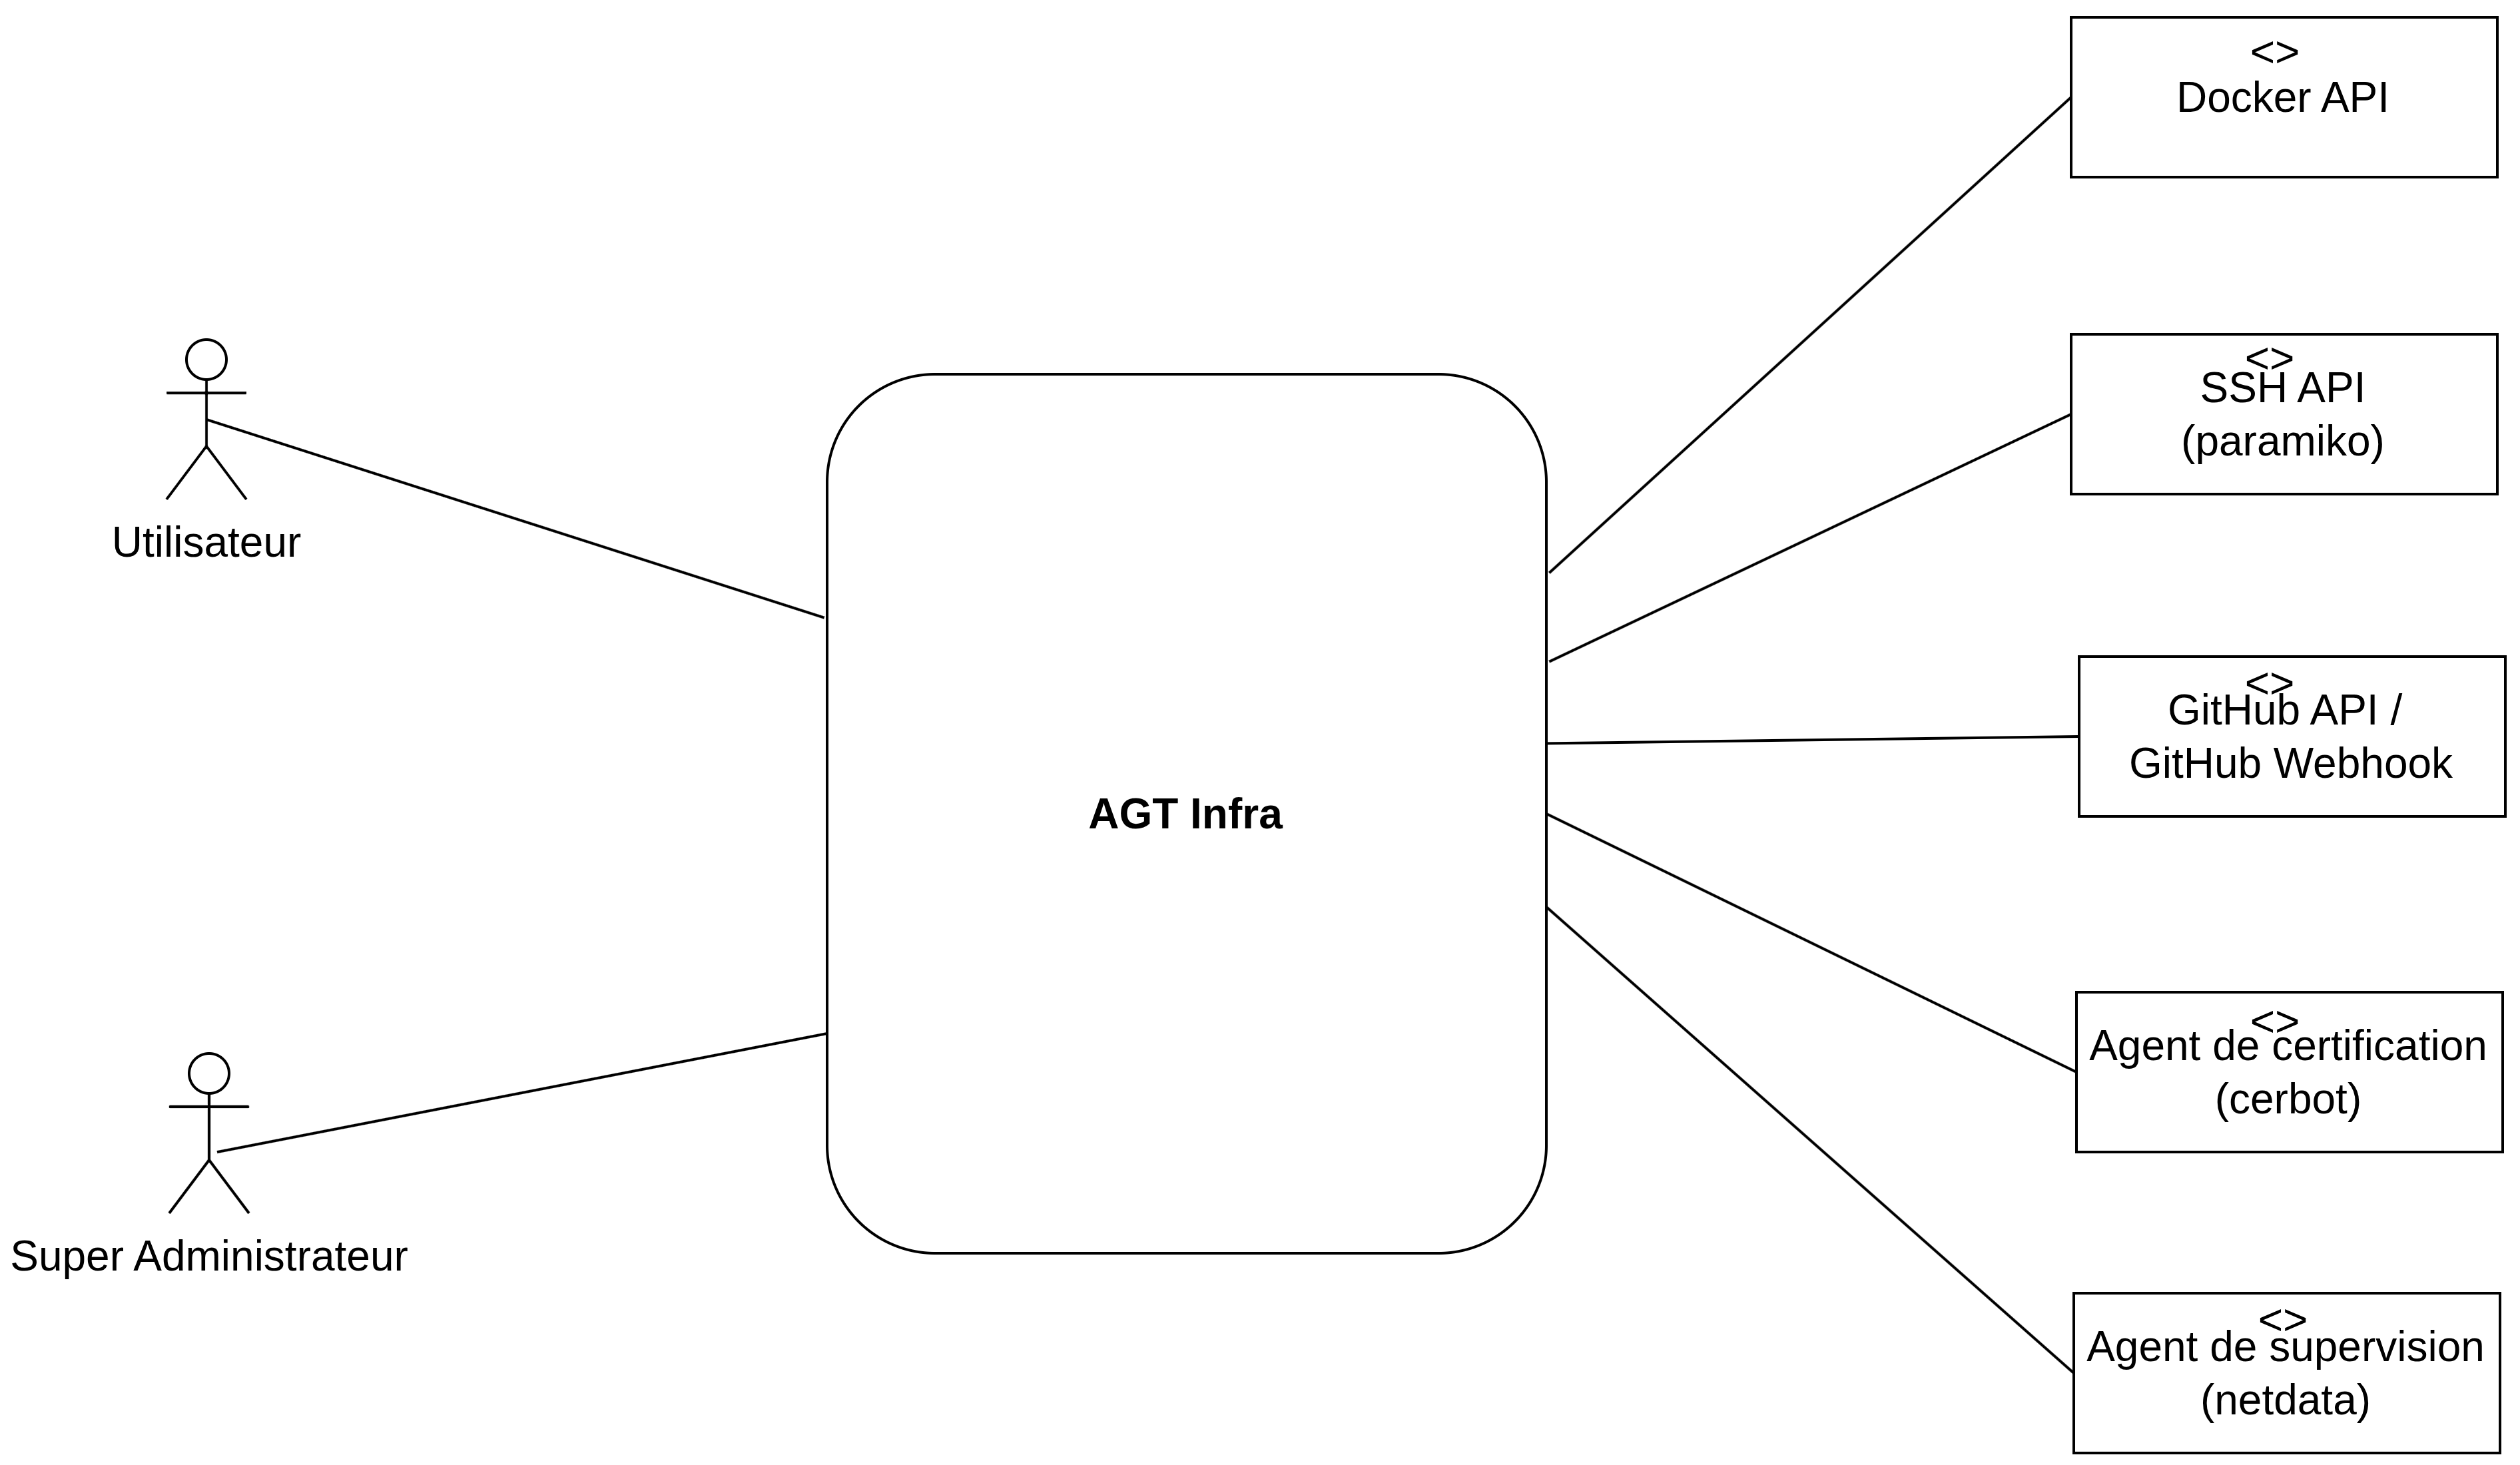
\includegraphics[width=0.85\linewidth]{assets/diagrams/03-diagramme_contexte.png}
  \caption{Diagramme de contexte d'AGT Infra}
  \label{fig:diagramme-contexte}
\end{figure}

Le périmètre fonctionnel réel se décompose en trois catégories.

\medskip
\noindent\textbf{Périmètre inclus} :
\begin{itemize}
  \item La gestion centralisée des serveurs physiques et des conteneurs
        Docker, avec une connectivité exclusivement fondée
        sur SSH.
  \item Le déploiement continu, la publication applicative sécurisée et
        la supervision des serveurs, à la demande comme en continu.
  \item Le contrôle d'accès dynamique et la traçabilité systématique de
        toute action sensible.
  \item La sauvegarde automatique de bases de données des application et
        volumes des conteneurs.
\end{itemize}

\medskip
\noindent\textbf{Périmètre exclu} :
\begin{itemize}
  \item La gestion des machines virtuelles et de l'hyperviseur associé.
  \item La montée en charge automatique et toute action corrective
        automatique d'un futur moteur de sécurité.
  \item La création automatique d'enregistrements DNS pour la publication
        applicative, qui reste une opération manuelle de l'utilisateur.
\end{itemize}

\medskip
\noindent\textbf{Contraintes transverses} :
\begin{itemize}
  \item La configurabilité indépendante de chaque mécanisme (déploiement,
        publication, supervision), activable ou désactivable sans effet
        de bord sur les autres.
  \item Le non-blocage de l'existant : l'adoption de l'outil reste
        progressive et n'empêche jamais un accès direct par SSH.
  \item L'absence de toute tâche de fond côté backend : toute collecte ou
        exécution part d'une action explicite.
\end{itemize}

\subsection{Acteurs}

Le système de rôles d'AGT Infra n'est pas figé : un seul rôle reste
immuable, tout le reste se compose librement.

\begin{itemize}
  \item \textbf{SUPER\_ADMIN} : rôle unique, présent dès l'installation,
        disposant d'un accès total, non révocable et jamais soumis à un
        refus explicite. Seul habilité à créer, modifier ou supprimer un
        rôle, à le composer à partir d'un catalogue de permissions, et à
        accorder ou refuser une permission directe à une personne
        précise.
  \item \textbf{Utilisateur} : toute autre personne, affectée à un rôle
        composé par un SUPER\_ADMIN. Son périmètre d'action dépend
        entièrement des permissions accordées à ce rôle et de la portée
        avec laquelle il lui a été attribué, globale ou restreinte à une
        ressource précise.
\end{itemize}

Ce modèle de contrôle d'accès dynamique sera détaillé plus loin dans ce
chapitre, lors de la modélisation des données.

\subsection{Synthèse des exigences par domaine}

Le tableau~\ref{tab:synthese-exigences} récapitule, domaine par domaine, ce
que couvre AGT Infra.

\begin{table}[H]
\centering
\small
\renewcommand{\arraystretch}{1.3}
\begin{tabular}{p{4.2cm}p{9.2cm}}
\toprule
\textbf{Domaine} & \textbf{Ce que couvre ce domaine} \\
\midrule
Serveurs physiques et connectivité SSH & Branchement, inventaire et
  authentification des serveurs par clé SSH dédiée, générée
  individuellement. \\
Conteneurs Docker et registres privés & Cycle de vie complet des
  conteneurs, avec possibilité de les créer depuis un registre privé isolé
  par utilisateur.\\
Environnements & Rattachement de chaque conteneur à un environnement
  préconfiguré (développement, test, production). \\
Console web & Session interactive sur un serveur ou un conteneur, avec
  enregistrement intégral du flux et relecture ultérieure. \\
Diagnostic à la demande et alertes & Collecte ponctuelle des métriques
  (CPU, RAM, disque) et déclenchement d'alertes en cas de dépassement de
  seuil. \\
Supervision continue & Surveillance autonome et permanente d'un serveur
  par un agent dédié, avec seuils et canaux de notification
  personnalisables. \\
Déploiement continu & Orchestration du déploiement d'une application à
  partir d'un dépôt Git, déclenché par un évènement vérifié. \\
Publication applicative & Exposition HTTPS d'une application déjà
  déployée, sous un nom de domaine. \\
Sauvegardes & Sauvegarde automatique, restaurable et vérifiée, des bases
  de données. \\
Montée en charge & Ajustement, dans un premier temps manuel, des
  ressources allouées à un conteneur. \\
Contrôle d'accès & Gestion des rôles et des permissions,
  pilotée en base de données plutôt que figée dans le code. \\
Sécurité & Vérification automatisée de règles de sécurité, limitée à
  l'audit et à la recommandation. \\
Journal d'audit & Traçabilité systématique de toute action sensible. \\
Documentation intégrée & Documentation d'exploitation consultable
  directement dans l'interface. \\
\bottomrule
\end{tabular}
\caption{Synthèse des exigences fonctionnelles par domaine}
\label{tab:synthese-exigences}
\end{table}

Ces exigences fonctionnelles sont complétées par des exigences non
fonctionnelles, transverses à l'ensemble des domaines. Elles se répartissent
en trois catégories.

\medskip
\noindent\textbf{Exigences vis-à-vis des utilisateurs} :
\begin{itemize}
  \item Aucun secret (clé SSH secrète, jeton, mot de passe) n'est jamais exposé en
        clair, y compris pour le rôle le plus privilégié.
  \item Chaque utilisateur reste isolé des secrets appartenant à un autre
        périmètre que le sien.
  \item Le déploiement, la publication et la supervision s'activent ou se
        désactivent indépendamment, sans effet de bord sur les autres.
\end{itemize}

\medskip
\noindent\textbf{Exigences organisationnelles (fonctionnement interne de
l'outil)} :
\begin{itemize}
  \item L'arrêt ou la panne d'un conteneur n'affecte jamais les autres
        conteneurs du même hôte.
  \item L'adoption de l'outil reste progressive : un accès direct demeure toujours possible en parallèle.
  \item Aucune tâche ne s'exécute de façon autonome côté serveur ; toute
        collecte ou exécution part d'une action explicite.
\end{itemize}

\medskip
\noindent\textbf{Exigences vis-à-vis des systèmes externes} :
\begin{itemize}
  \item AGT Infra pilote des briques déjà éprouvées (Docker, SSH, Nginx,
        Certbot, GitHub) sans jamais les réimplémenter.
  \item La fiabilité d'une sauvegarde dépend d'une restauration
        effectivement vérifiée sur une cible de test.
\end{itemize}

\subsection{Diagramme de cas d'utilisation}

Plutôt qu'un diagramme unique regroupant les cas d'utilisation des
quatorze domaines, ce qui nuirait à sa lisibilité, deux diagrammes
illustrent ici les domaines concentrant le plus d'interactions entre
acteurs et système. \\
Le premier diagramme (figure~\ref{fig:cas-utilisation-rbac}) porte sur le
domaine du contrôle d'accès.

\begin{figure}[H]
  \centering
  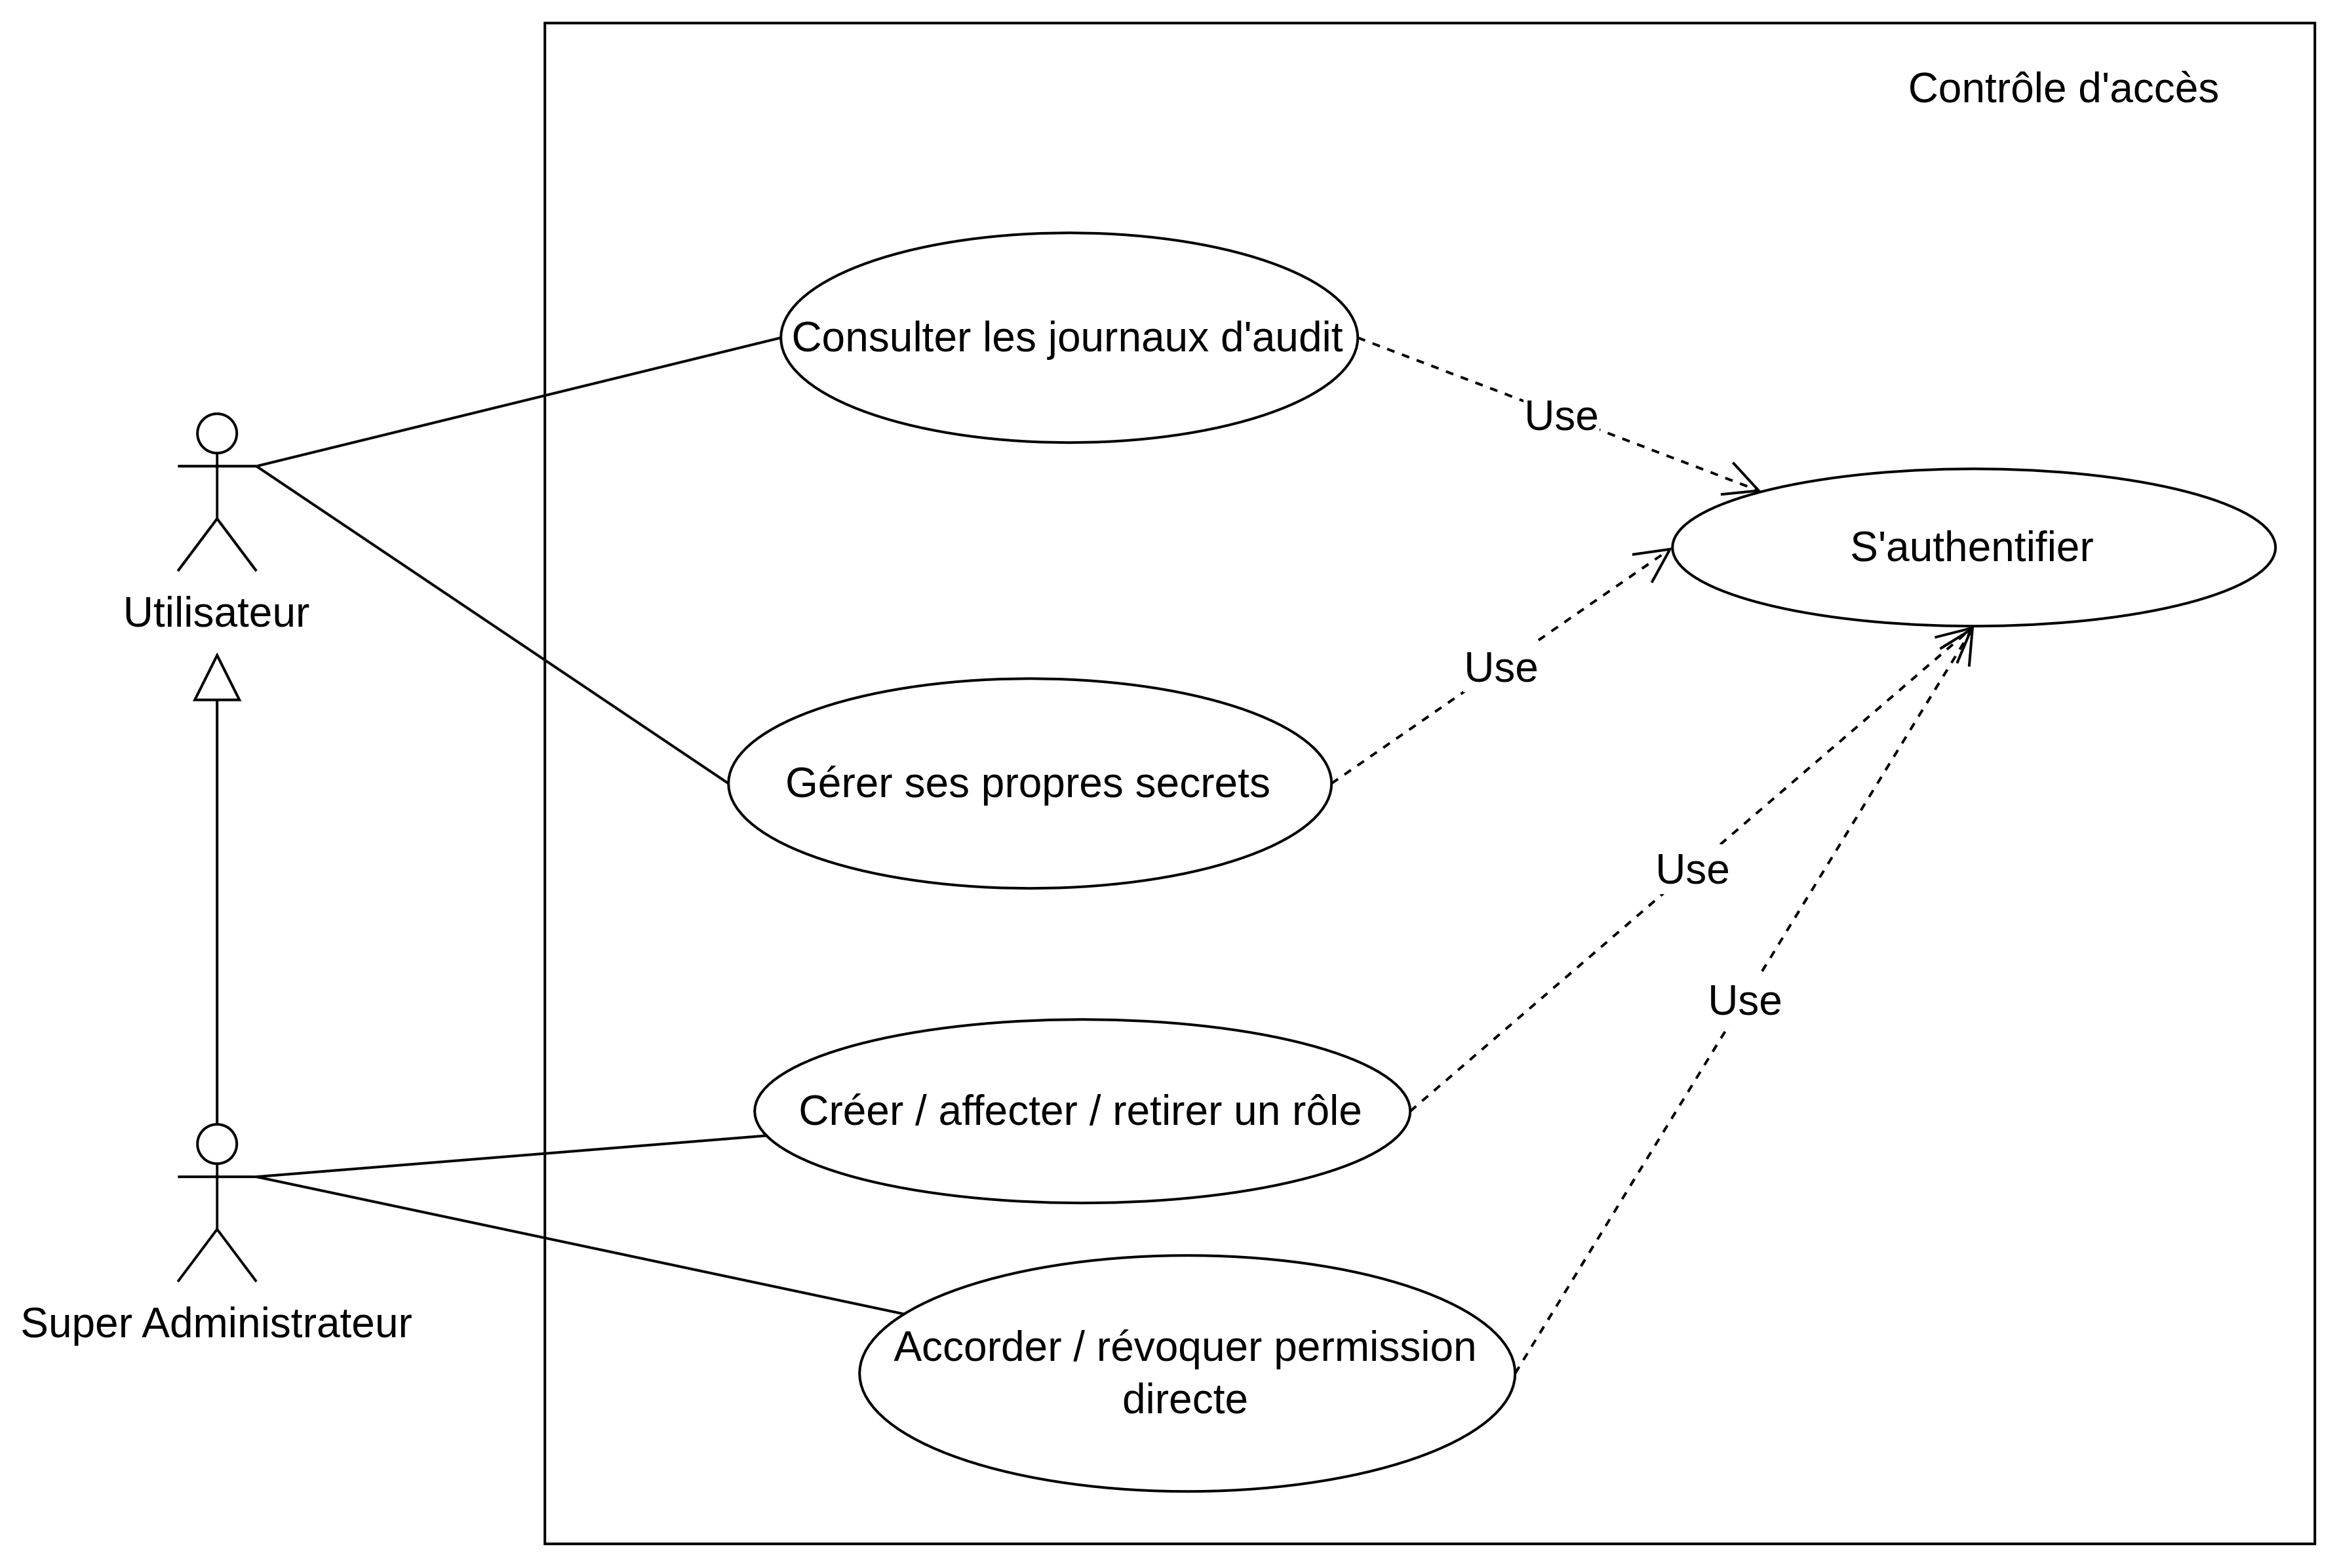
\includegraphics[width=0.85\linewidth]{assets/diagrams/03-diagramme_cas_utilisation_RBAC.png}
  \caption{Diagramme de cas d'utilisation, domaine Contrôle d'accès}
  \label{fig:cas-utilisation-rbac}
\end{figure}

Le second diagramme (figure~\ref{fig:cas-utilisation-serveurs}) porte sur
le domaine des serveurs et conteneurs. Il illustre la dépendance du
système envers les briques externes qu'il orchestre.

\begin{figure}[H]
  \centering
  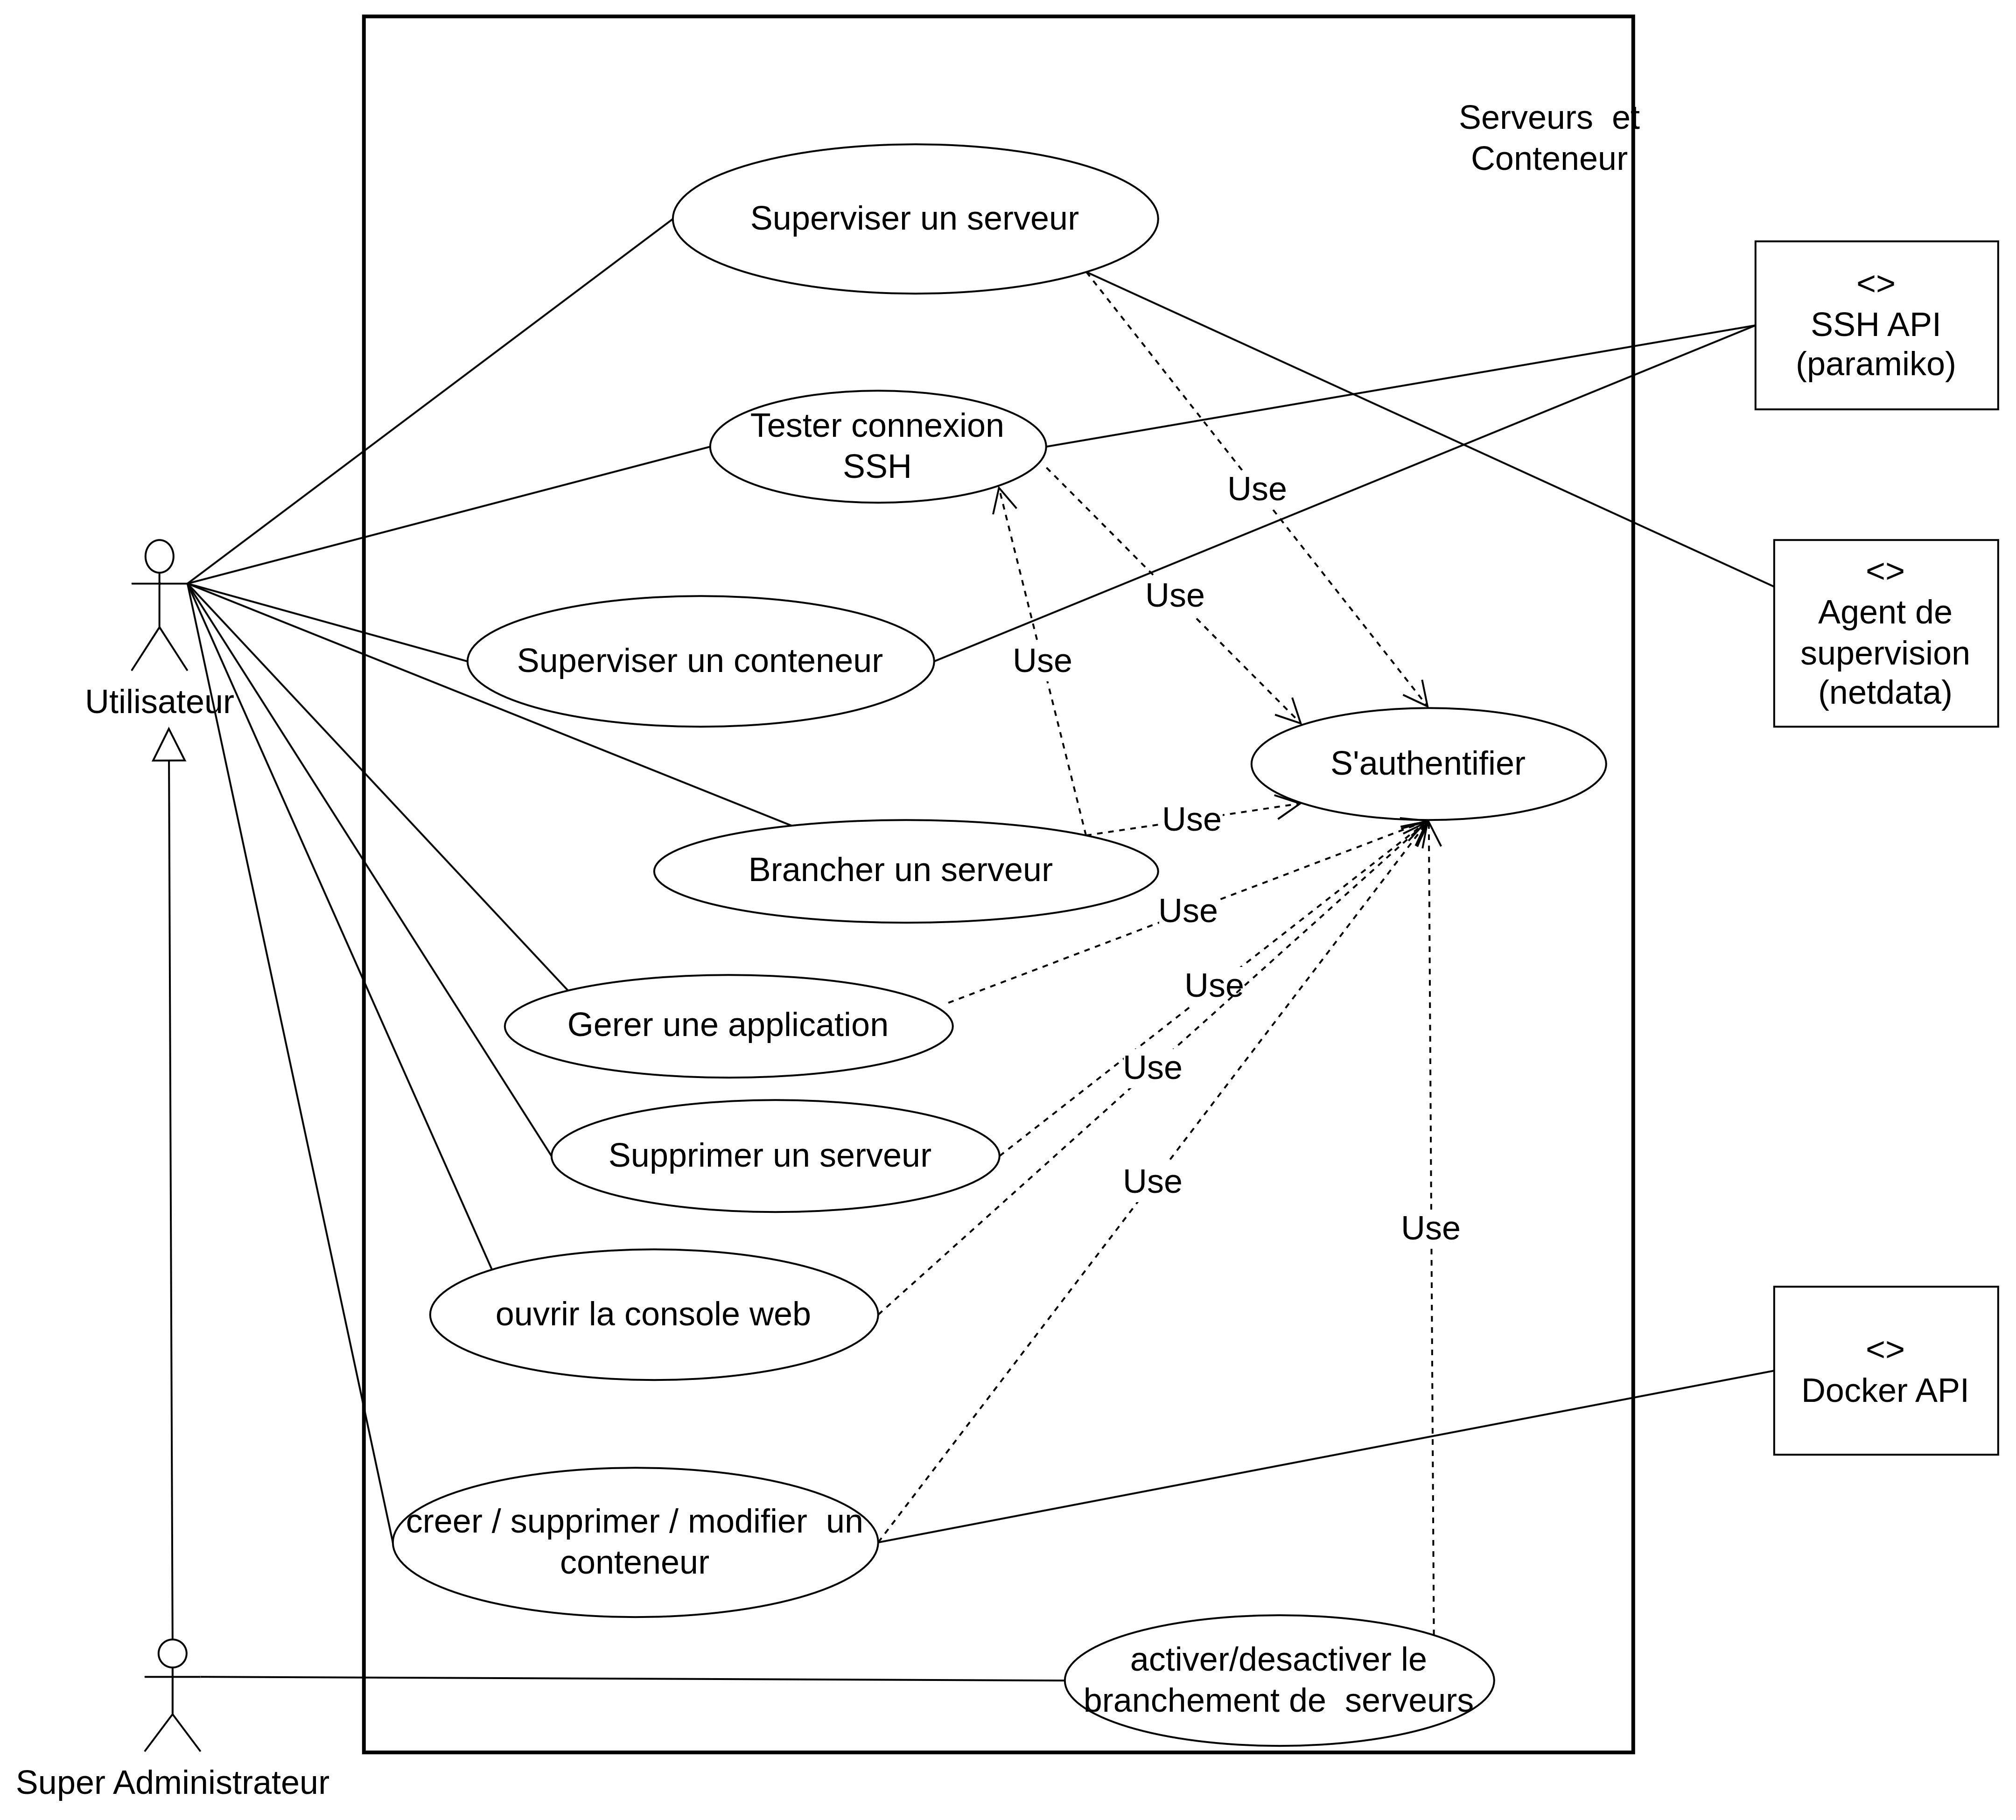
\includegraphics[width=0.85\linewidth]{assets/diagrams/03-diagramme_cas_utilisation_SERVEUR-CONTENEUR.png}
  \caption{Diagramme de cas d'utilisation, domaine Serveurs et conteneurs}
  \label{fig:cas-utilisation-serveurs}
\end{figure}

\subsection{Quelques cas d'utilisation détaillés}

Les deux cas d'utilisation suivants,sont détaillés pour donner un exemple concret de scénario
nominal et de scénarios alternatifs.

\paragraph{Créer et affecter un rôle}
\begin{itemize}
  \item \textbf{Acteur principal} : le SUPER\_ADMIN.
  \item \textbf{Acteurs secondaires} : aucun système externe, l'opération
        reste interne à AGT Infra.
  \item \textbf{Objectif} : le SUPER\_ADMIN veut composer un rôle à partir
        d'un sous-ensemble de permissions, puis l'affecter à une personne,
        afin de lui donner un périmètre d'action précis sans lui accorder
        un accès total.
  \item \textbf{Préconditions} :
        \begin{itemize}
          \item Le SUPER\_ADMIN est authentifié.
          \item La personne à qui le rôle sera affecté possède déjà un
                compte sur AGT Infra.
        \end{itemize}
  \item \textbf{Postconditions} : la personne dispose du nouveau rôle, et
        son périmètre d'action reflète immédiatement les permissions qui
        lui ont été accordées.
  \item \textbf{Scénario nominal} :
        \begin{enumerate}
          \item Le SUPER\_ADMIN ouvre l'écran de gestion des rôles.
          \item Il sélectionne, dans le catalogue de permissions, celles
                qu'il souhaite regrouper dans un nouveau rôle.
          \item Il nomme ce rôle et confirme sa création.
          \item Il affecte ce rôle à la personne concernée, en précisant
                une portée globale ou restreinte à une ressource précise.
        \end{enumerate}
  \item \textbf{Scénarios alternatifs} :
        \begin{itemize}
          \item Le SUPER\_ADMIN tente de retirer un droit au rôle
                SUPER\_ADMIN lui-même : l'opération est refusée, ce rôle
                restant immuable.
          \item Une permission accordée au rôle est par ailleurs
                explicitement refusée à cette personne à titre individuel :
                le refus prévaut, et l'action reste bloquée pour elle
                malgré le rôle qui l'autoriserait.
        \end{itemize}
\end{itemize}

\paragraph{Déployer une application}
\begin{itemize}
  \item \textbf{Acteur principal} : l'Utilisateur.
  \item \textbf{Acteurs secondaires} : GitHub, à l'origine de l'évènement
        déclencheur ; l'API SSH (Paramiko), sollicitée pour exécuter le
        déploiement sur le serveur cible ; Docker, sollicité pour la
        construction et le démarrage du conteneur.
  \item \textbf{Objectif} : déployer une nouvelle version d'une
        application, depuis la modification du code jusqu'à son exécution
        effective sur le serveur cible, avec un suivi en direct de chaque
        étape.
  \item \textbf{Préconditions} :
        \begin{itemize}
          \item Une configuration de déploiement existe déjà pour ce
                dépôt (branche, environnement, serveur cible, secret de
                webhook).
          \item Le déploiement automatique est activé pour cette configuration.
        \end{itemize}
  \item \textbf{Postconditions} : l'application est opérationnelle sur le
        serveur cible, et l'intégralité du déroulement du déploiement
        reste consultable dans l'historique.
  \item \textbf{Scénario nominal} :
        \begin{enumerate}
          \item Une modification poussée sur le dépôt GitHub configuré déclenche
                un évènement webhook vers AGT Infra.
          \item AGT Infra vérifie l'authenticité de cet évènement par
                validation de sa signature.
          \item La configuration de déploiement correspondante est
                identifiée et chargée.
          \item Un job de déploiement démarre son exécution sur le
                serveur cible via SSH, selon une séquence de huit étapes :
                connexion SSH, vérifications préalables, synchronisation
                du dépôt Git, génération des variables d'environnement de l'application,
                construction de l'image Docker, démarrage du conteneur,
                vérification de bon fonctionnement, puis nettoyage des
                ressources temporaires.
          \item Chaque étape écrit sa progression dans un journal au fil
                de l'eau, diffusé en temps réel sur un canal dédié.
          \item L'Utilisateur suit le déploiement en direct depuis la
                console de déploiement de l'interface AGT Infra.
        \end{enumerate}
  \item \textbf{Scénarios alternatifs} :
        \begin{itemize}
          \item La signature de l'évènement webhook ne peut pas être
                validée : l'évènement est rejeté et journalisé, sans
                aucune exécution.
          \item Une étape de la séquence échoue, par exemple la
                vérification de bon fonctionnement du conteneur : le
                déploiement est interrompu, marqué comme échoué, et les
                étapes suivantes ne sont pas exécutées.
          \item Le déploiement automatique est désactivé pour cette configuration :
                l'évènement est reçu et journalisé, mais n'entraîne aucune
                exécution.
        \end{itemize}
\end{itemize}





\section{Architecture générale}

L'analyse des besoins ayant établi ce que le système doit accomplir,
cette section décrit comment il est structuré pour y répondre : ses
grandes parties, leurs responsabilités respectives, et la façon dont
elles communiquent entre elles.

\subsection{Architecture logique}

Le diagramme de la figure~\ref{fig:architecture-globale} distingue
nettement deux ensembles : à gauche, les composants internes à AGT
Infra ; à droite, les systèmes externes qu'il orchestre sans jamais les
réimplémenter, conformément au principe de chef d'orchestre déjà énoncé
dans l'introduction de ce rapport.

\begin{figure}[H]
  \centering
  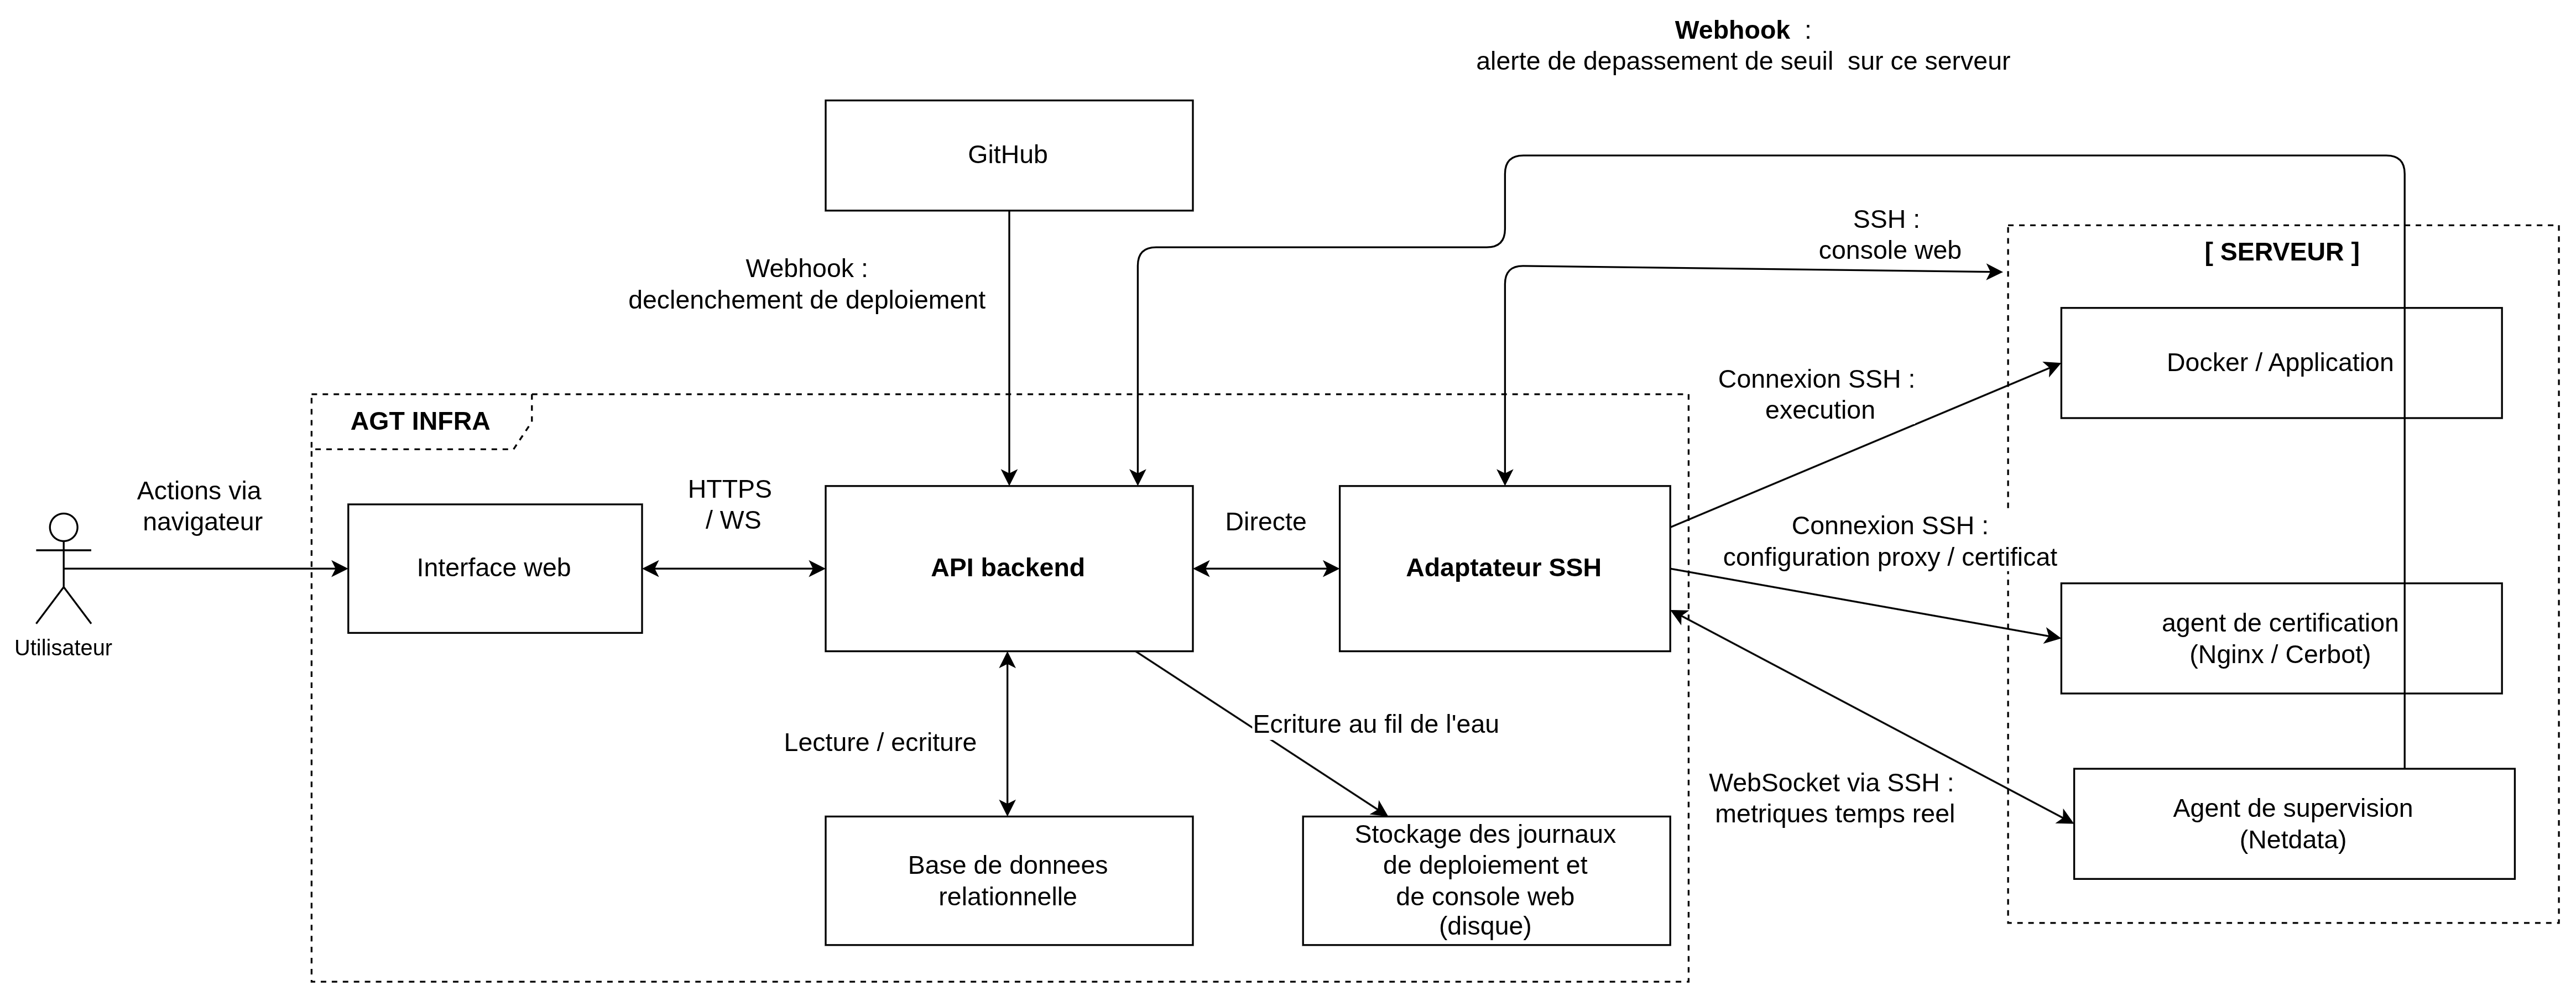
\includegraphics[width=\linewidth]{assets/diagrams/03-diagramme_architecture-globale.png}
  \caption{Architecture générale d'AGT Infra}
  \label{fig:architecture-globale}
\end{figure}

L'Utilisateur n'accède jamais directement à une ressource sensible :
toute action passe par l'interface web, qui communique avec l'API
backend en HTTPS et via un canal WebSocket dédié pour les flux temps
réel (journaux de déploiement, console web). Seule l'API backend décide
si une action est autorisée, selon le modèle RBAC/IBAC ; ni l'interface
web ni l'adaptateur SSH ne portent cette logique, le premier se limitant
à l'affichage, le second à l'exécution des commandes déléguées.

Toute opération sur un serveur distant transite par ce même adaptateur
SSH, qu'il s'agisse d'une commande Docker, d'une configuration Nginx/
Certbot, ou d'un canal WebSocket vers l'agent de supervision. Seule
exception : l'agent Netdata notifie l'API backend directement par
webhook en cas de dépassement de seuil, ce qui permet à une alerte de se
déclencher même sans consultation en cours.

La persistance suit deux logiques distinctes : la base de données
relationnelle porte les données structurées du système (utilisateurs,
rôles, permissions, serveurs, conteneurs, publications), tandis que les
journaux de déploiement et les sessions de console web sont écrits
directement sur disque au fil de l'exécution, la base n'en conservant
qu'une synthèse consultable.

\subsection{Diagramme de package}

Le diagramme de package de la figure~\ref{fig:diagramme-package} détaille
l'organisation interne d'AGT Infra en grands domaines fonctionnels, sans
descendre au niveau des classes. Chaque flèche en pointillé, annotée
\textit{Use}, indique qu'un package dépend d'un autre pour fonctionner.

\begin{figure}[H]
  \centering
  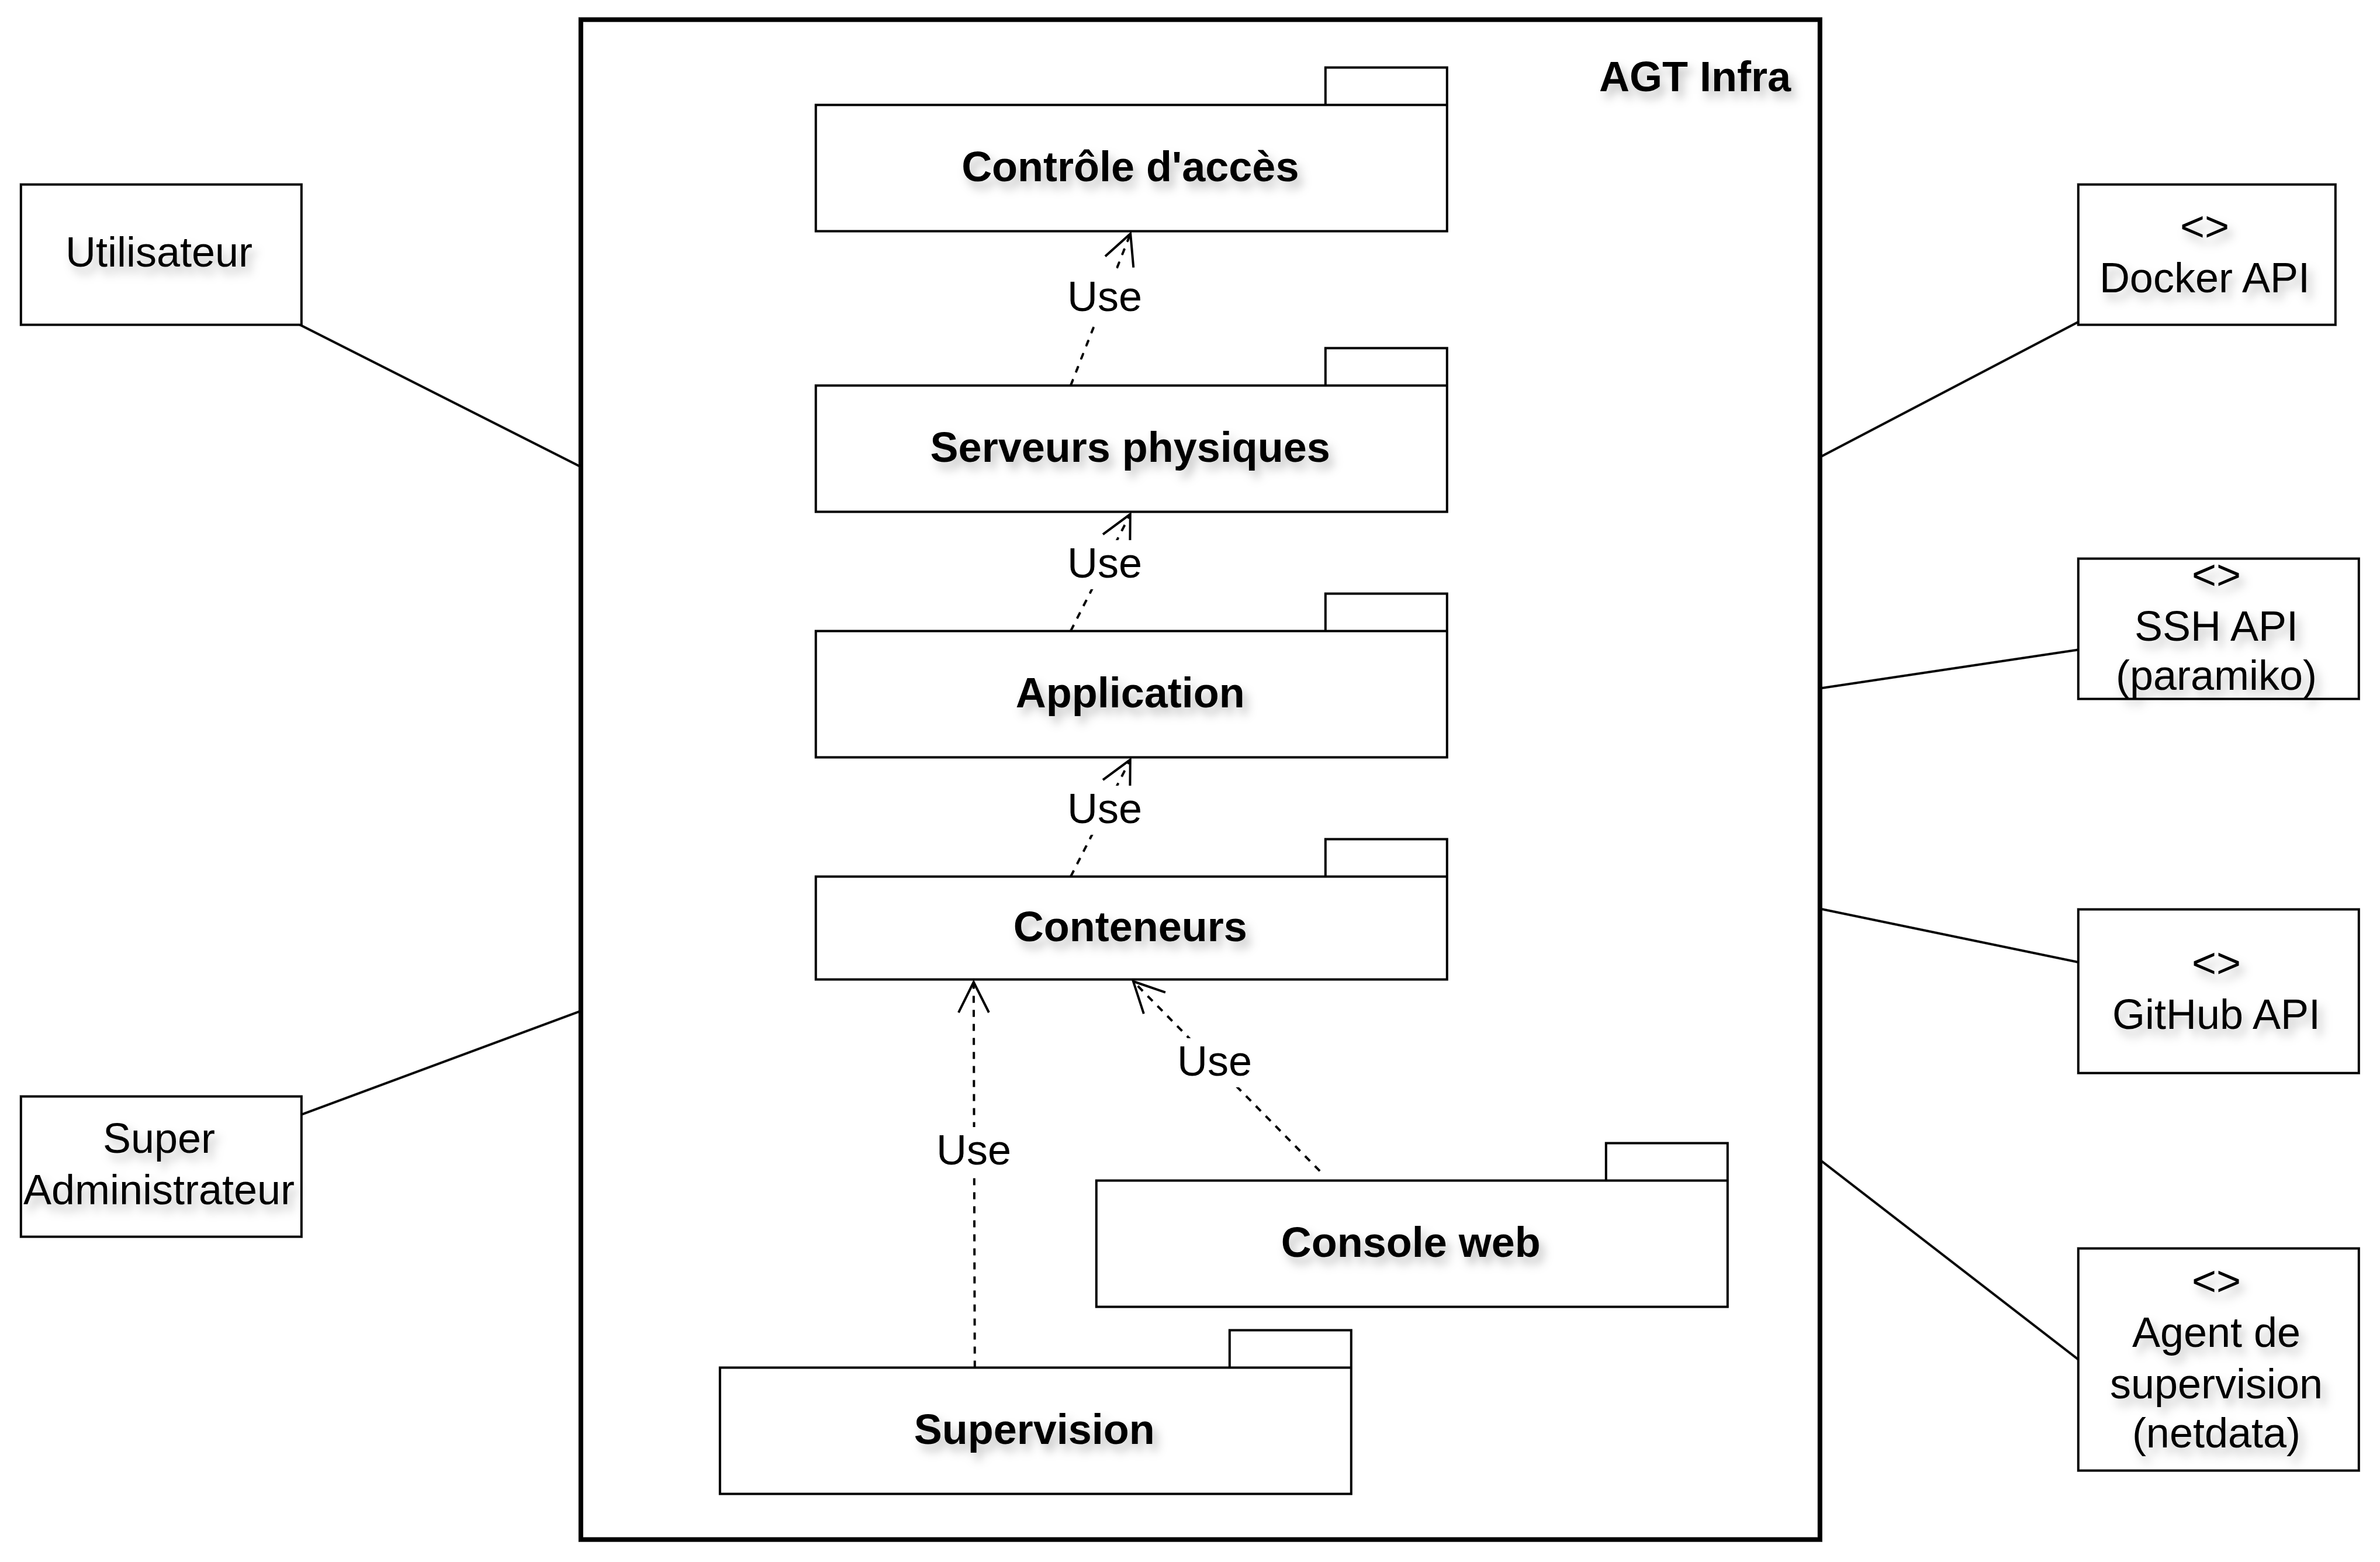
\includegraphics[width=0.85\linewidth]{assets/diagrams/03-diagramme_packages.png}
  \caption{Diagramme de package d'AGT Infra}
  \label{fig:diagramme-package}
\end{figure}

Le package Contrôle d'accès occupe une position particulière : il n'est
utilisé que par le package Serveurs physiques, mais toute action menée
depuis n'importe quel autre package du système passe en réalité par une
vérification de permission avant de s'exécuter, cette dépendance
transverse n'étant pas répétée sur chaque package pour ne pas surcharger
le diagramme. Les packages Serveurs physiques, Application et Conteneurs
s'enchaînent ensuite de façon hiérarchique, chacun reposant sur le
précédent, jusqu'aux packages Supervision et Console web, qui dépendent
tous deux du package Conteneurs pour cibler la ressource sur laquelle ils
opèrent.

Sur la droite du diagramme apparaissent les interfaces externes
sollicitées par ces packages : l'API Docker pour la gestion des
conteneurs, l'API SSH (Paramiko) pour toute connexion distante, l'API
GitHub pour la réception des évènements de déploiement, et l'agent de
supervision Netdata pour la collecte continue des métriques.

\section{Modélisation des données}

Cette section modélise les entités qui portent, au niveau des données,
les décisions déjà présentées : le contrôle d'accès d'une part, la
gestion des serveurs et des conteneurs d'autre part. Comme pour les cas
d'utilisation, deux diagrammes de classes illustrent ces domaines,
plutôt qu'un schéma unique regroupant l'ensemble du système.

\subsection{Modèle du contrôle d'accès (RBAC/IBAC)}

\begin{figure}[H]
  \centering
  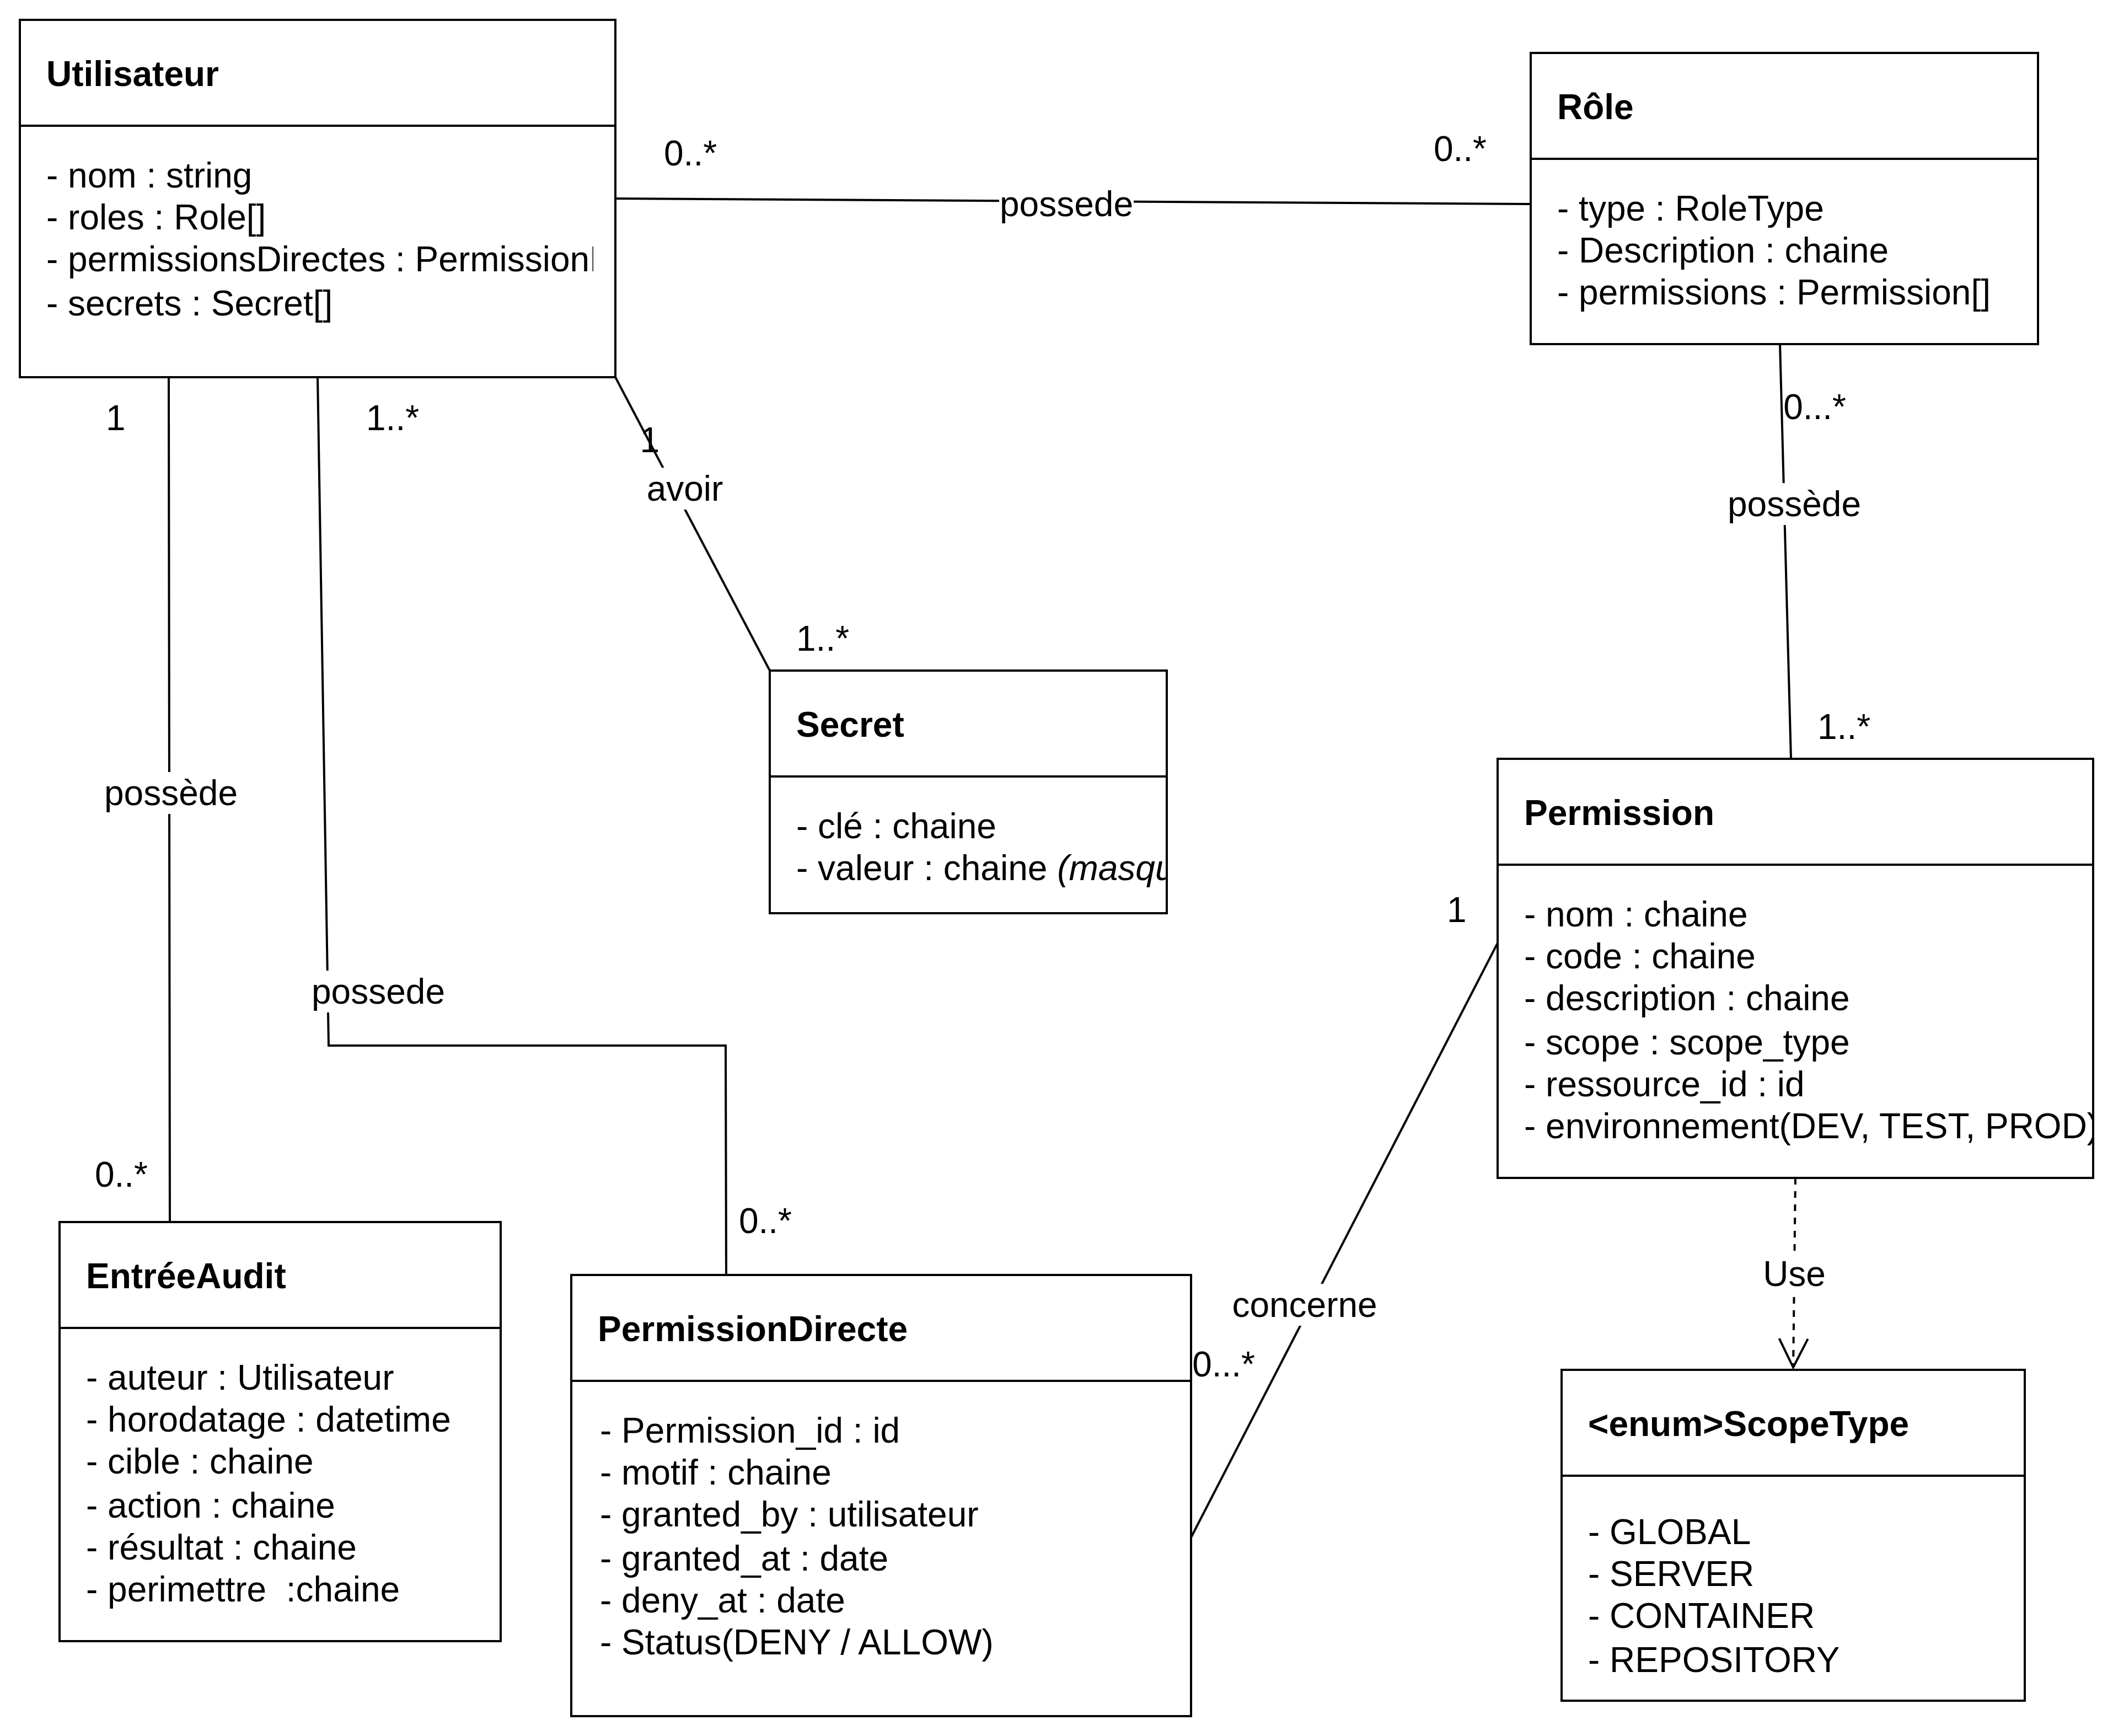
\includegraphics[width=\linewidth]{assets/diagrams/03-diagramme_classe_acces.png}
  \caption{Diagramme de classes, domaine Contrôle d'accès}
  \label{fig:diagramme-classe-acces}
\end{figure}

Un Utilisateur possède plusieurs Rôles, chacun regroupant un ensemble de
Permission choisies dans un catalogue commun. Chaque Permission porte une
portée (scope), globale ou restreinte à un serveur, un conteneur ou un
registre, conformément au modèle déjà évoqué dans l'analyse des besoins.

Une PermissionDirecte accorde ou refuse une Permission précise à un
Utilisateur précis, indépendamment de ses rôles, avec son propre motif et
son propre statut (\textit{allow} ou \textit{deny}). C'est cette classe
qui porte, au niveau des données, le principe de refus explicite toujours
prioritaire déjà énoncé plus haut.

Chaque Utilisateur possède également ses propres Secret, dont la valeur
reste masquée, et peut être l'auteur de plusieurs EntréeAudit, chacune
traçant une action précise : sa cible, son résultat et son périmètre.

\subsection{Modèle des serveurs et des conteneurs}

\begin{figure}[H]
  \centering
  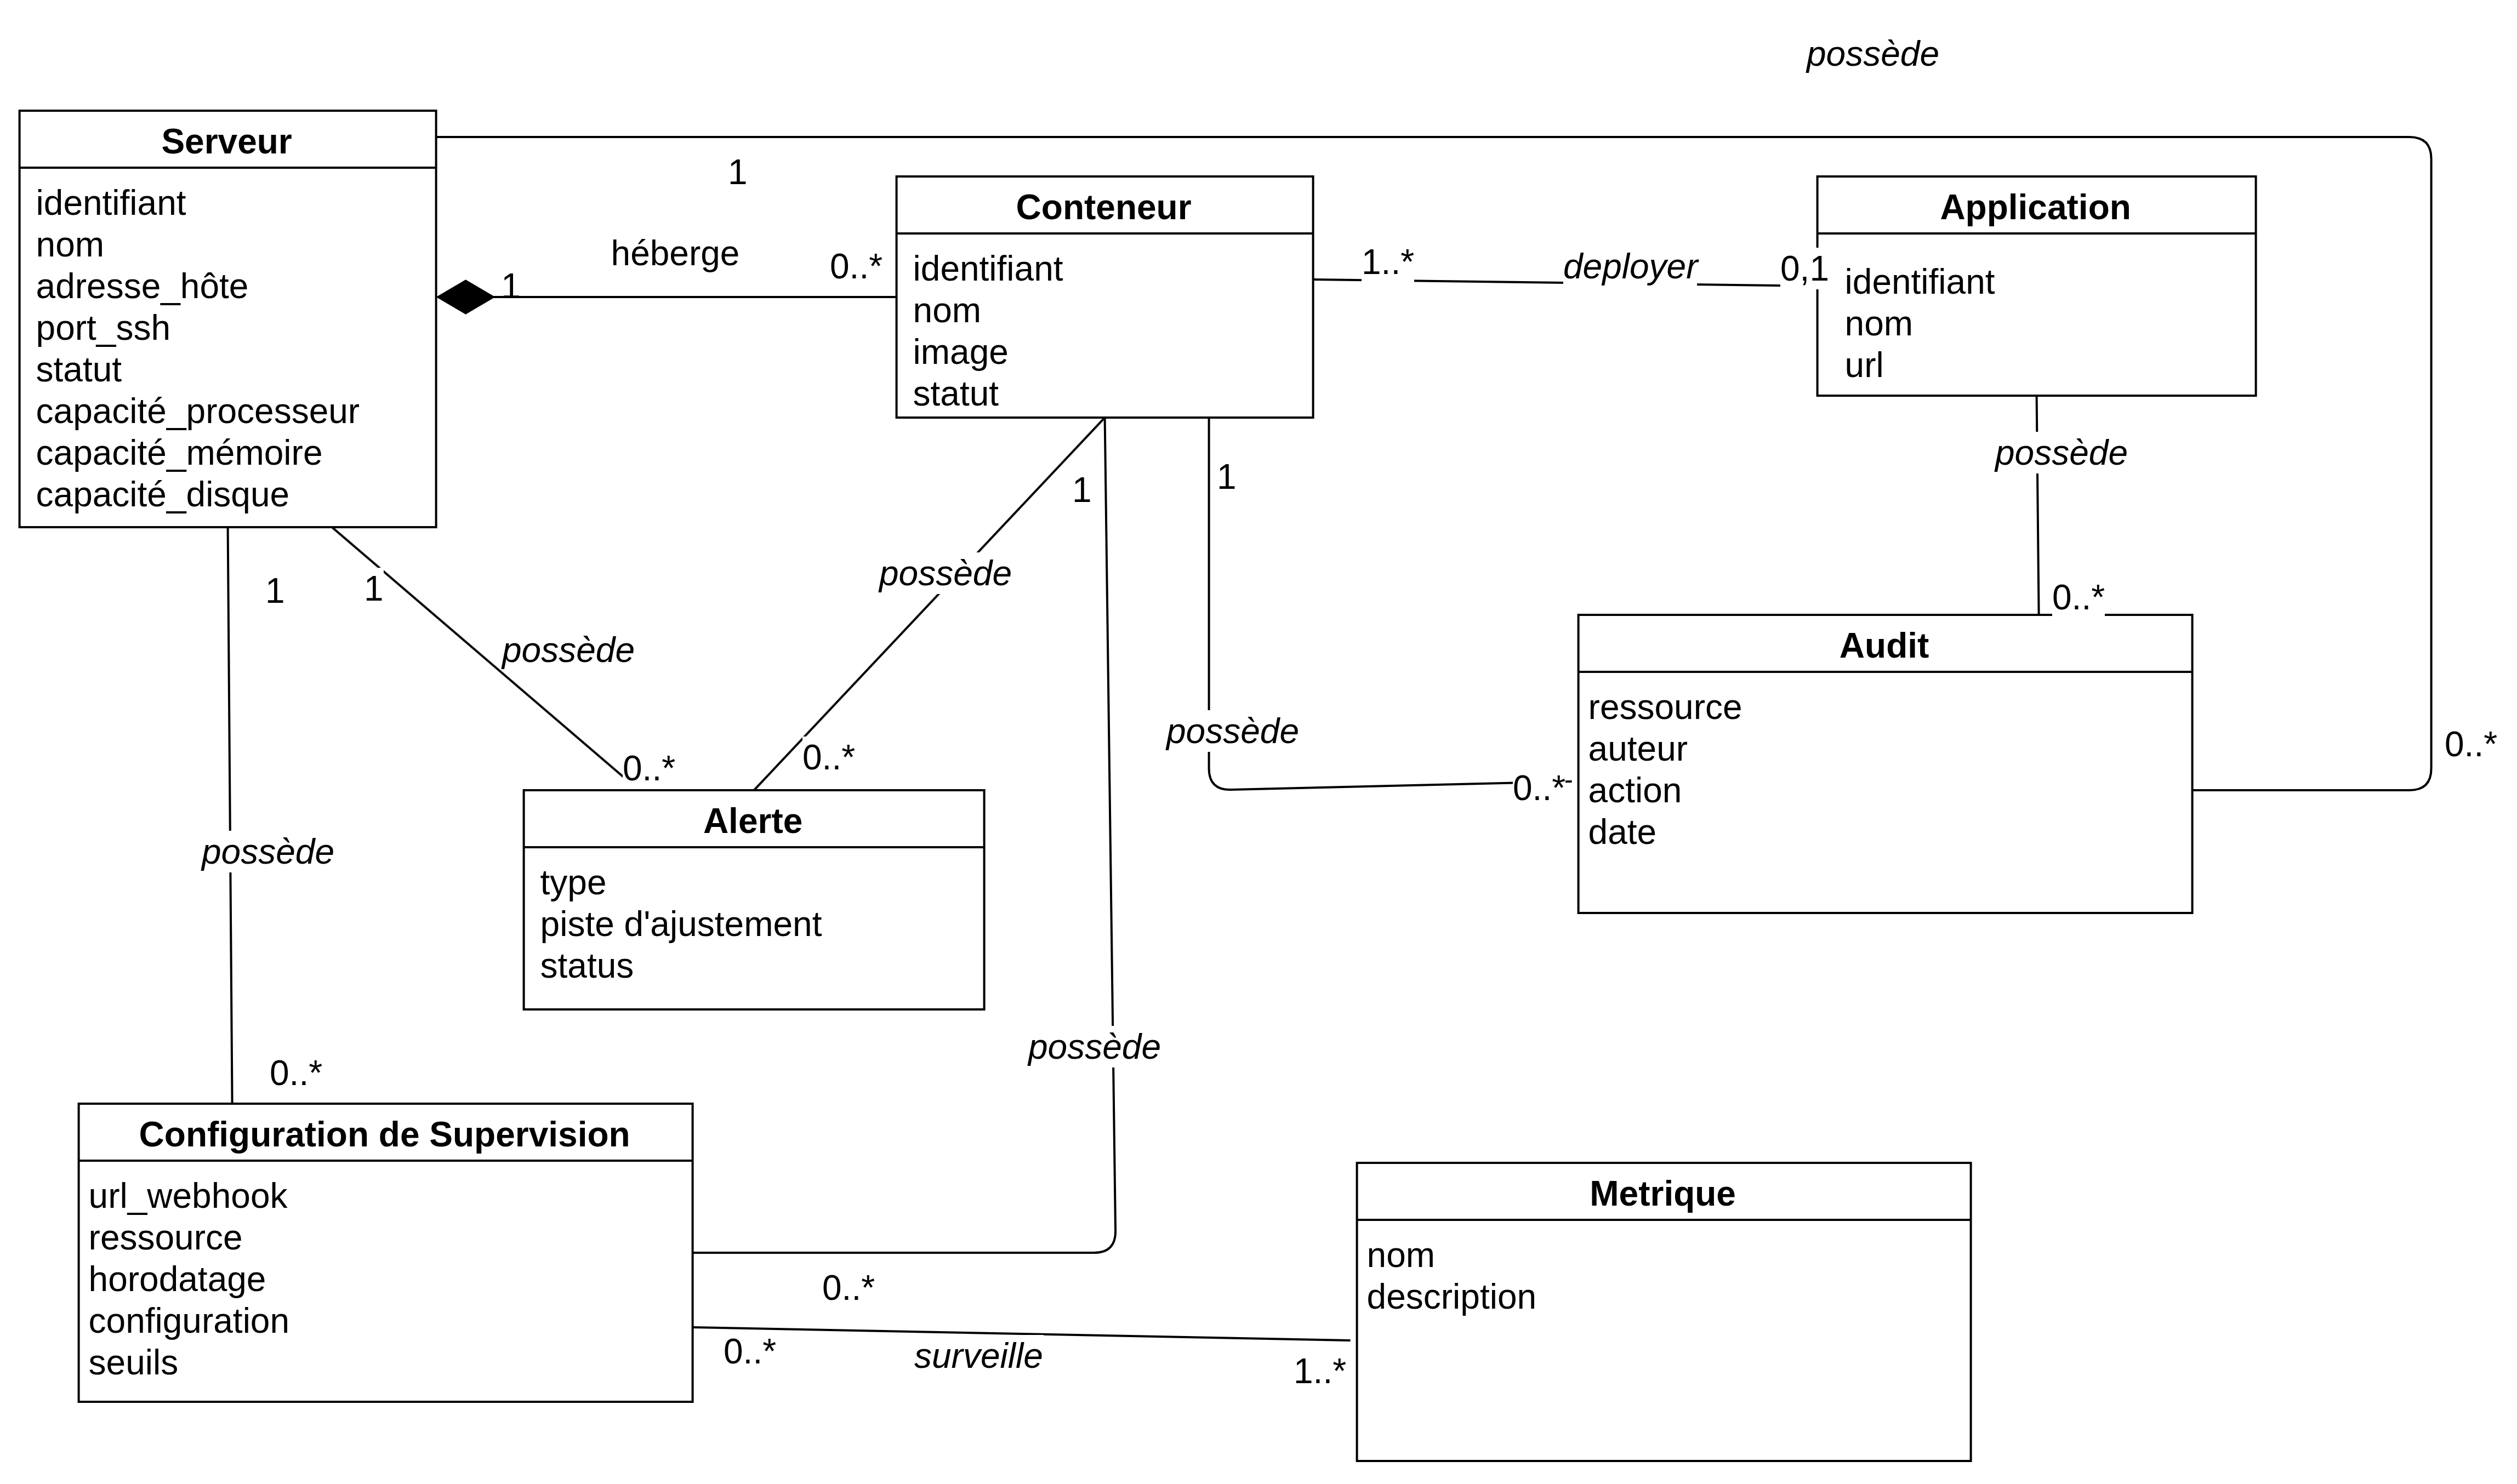
\includegraphics[width=\linewidth]{assets/diagrams/03-diagramme_classe_srv_cnt.png}
  \caption{Diagramme de classes, domaine Serveurs et conteneurs}
  \label{fig:diagramme-classe-srv-cnt}
\end{figure}

Un Serveur héberge plusieurs Conteneurs, chacun pouvant être associé à une
Application qui y est déployée, cette association restant facultative.
Serveurs et conteneurs peuvent l'un comme l'autre déclencher plusieurs
Alerte et faire l'objet de plusieurs entrées Audit.

Une Configuration de Supervision, rattachée à un serveur, définit les
seuils et le point de notification utilisés pour surveiller un ensemble
de Metrique propres à ce serveur.

La section suivante s'appuie sur ce modèle pour détailler deux
comportements clés du système : le cycle de vie d'une publication, et
l'algorithme de résolution d'une permission.

\section{Comportements clés}

Cette dernière section de l'analyse et de la conception détaille cinq
comportements du système, choisis parce qu'ils illustrent chacun une
règle de gestion déjà énoncée dans ce chapitre plutôt que par
exhaustivité. Deux diagrammes d'état-transition montrent le cycle de vie
d'une publication et celui de la connectivité d'un serveur ; trois
diagrammes de séquence détaillent des échanges entre systèmes déjà
introduits en tant que cas d'utilisation.

\subsection{Cycle de vie d'une publication applicative}

\begin{figure}[H]
  \centering
  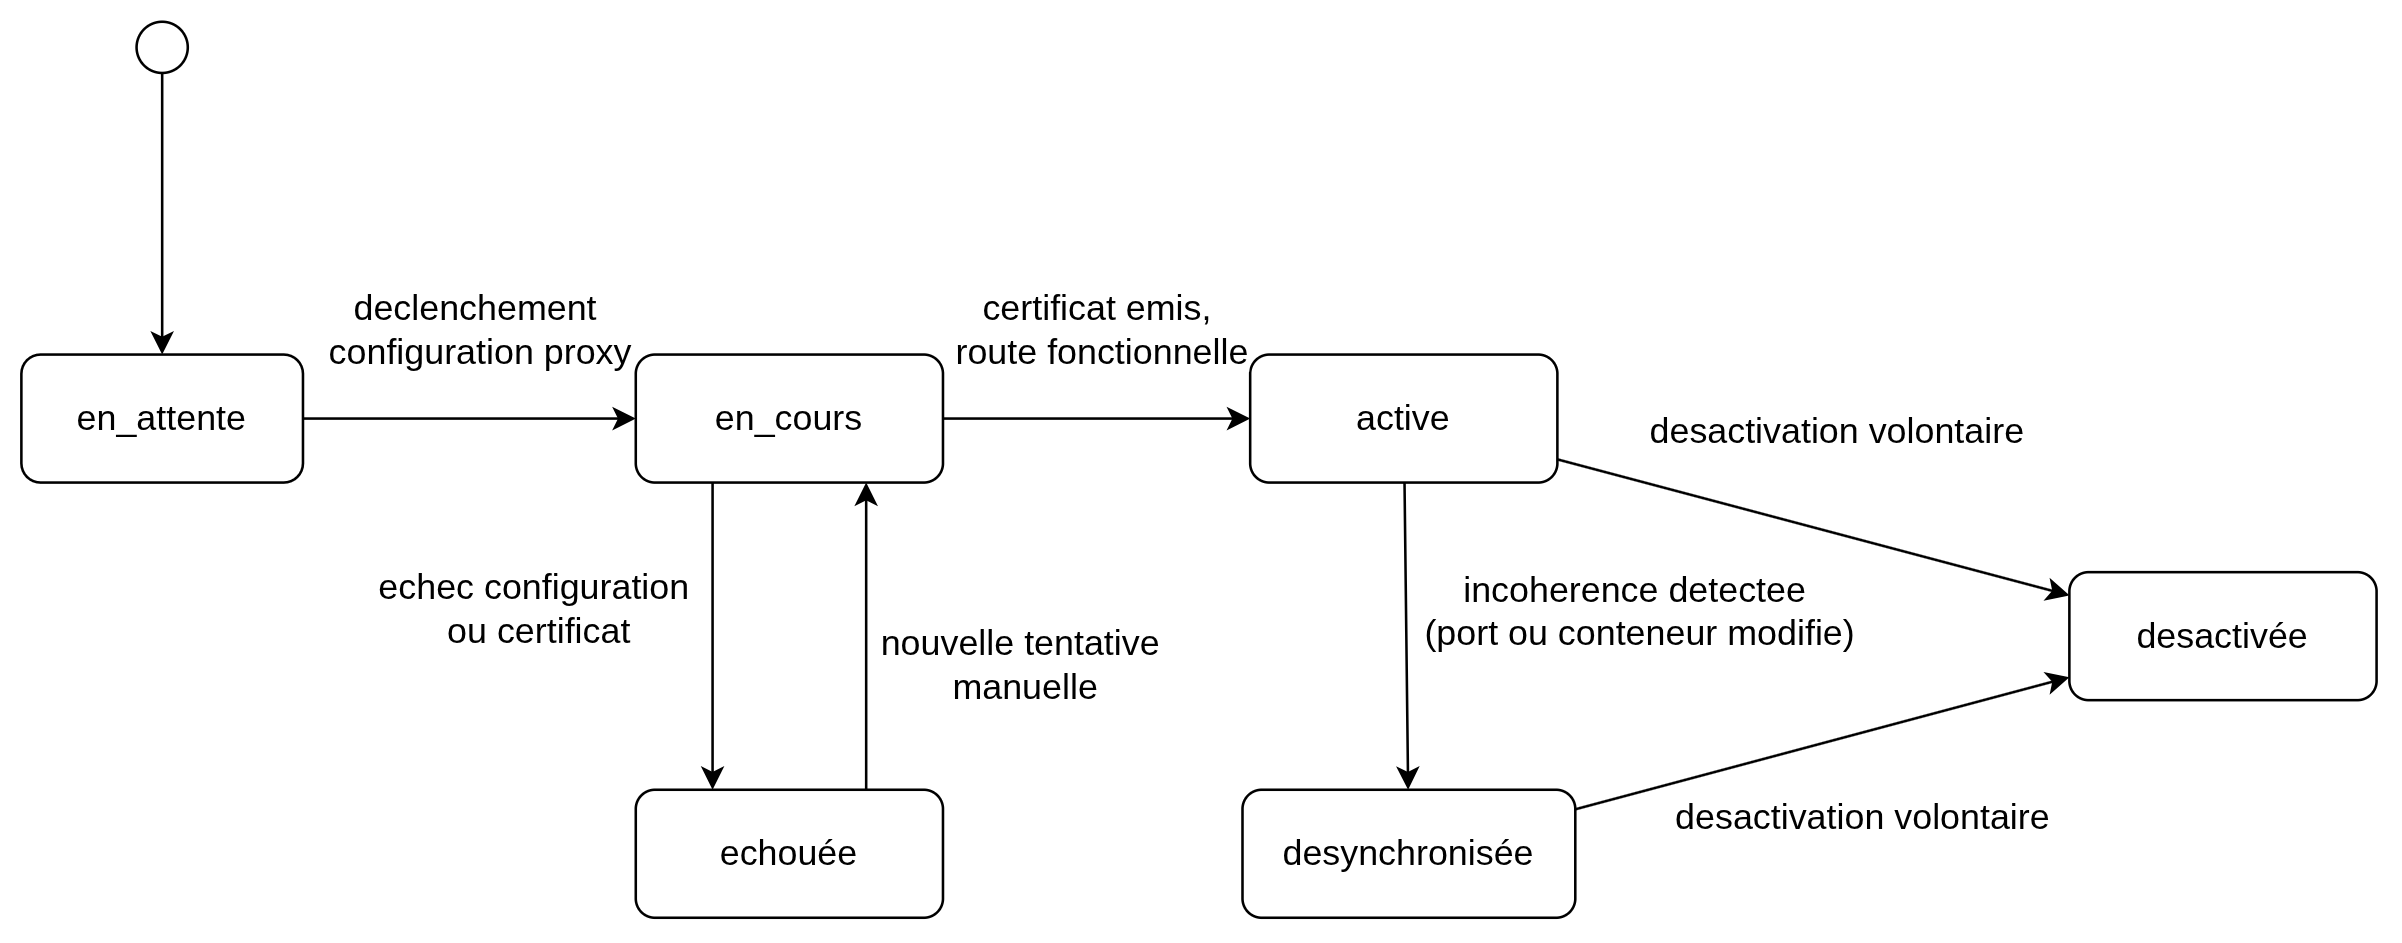
\includegraphics[width=\linewidth]{assets/diagrams/03-diagramme_ET_publication.png}
  \caption{État-transition d'une publication applicative}
  \label{fig:etat-publication}
\end{figure}

Une publication traverse six états. Le point à retenir se situe dans les
deux états d'échec :

\begin{itemize}
  \item \texttt{echouée} peut être relancée manuellement, ce qui la
        ramène en \texttt{en\_cours}.
  \item \texttt{desynchronisée}, en revanche, ne revient jamais
        automatiquement à \texttt{active} : une incohérence détectée
        (port ou conteneur modifié) reste signalée jusqu'à intervention
        volontaire de l'utilisateur.
\end{itemize}

Cette absence de correction automatique est un choix délibéré, déjà
justifié dans le cahier des charges : une publication corrigée seule
masquerait un changement de configuration que l'utilisateur doit
explicitement valider.

\subsection{Cycle de vie de la connectivité d'un serveur}

\begin{figure}[H]
  \centering
  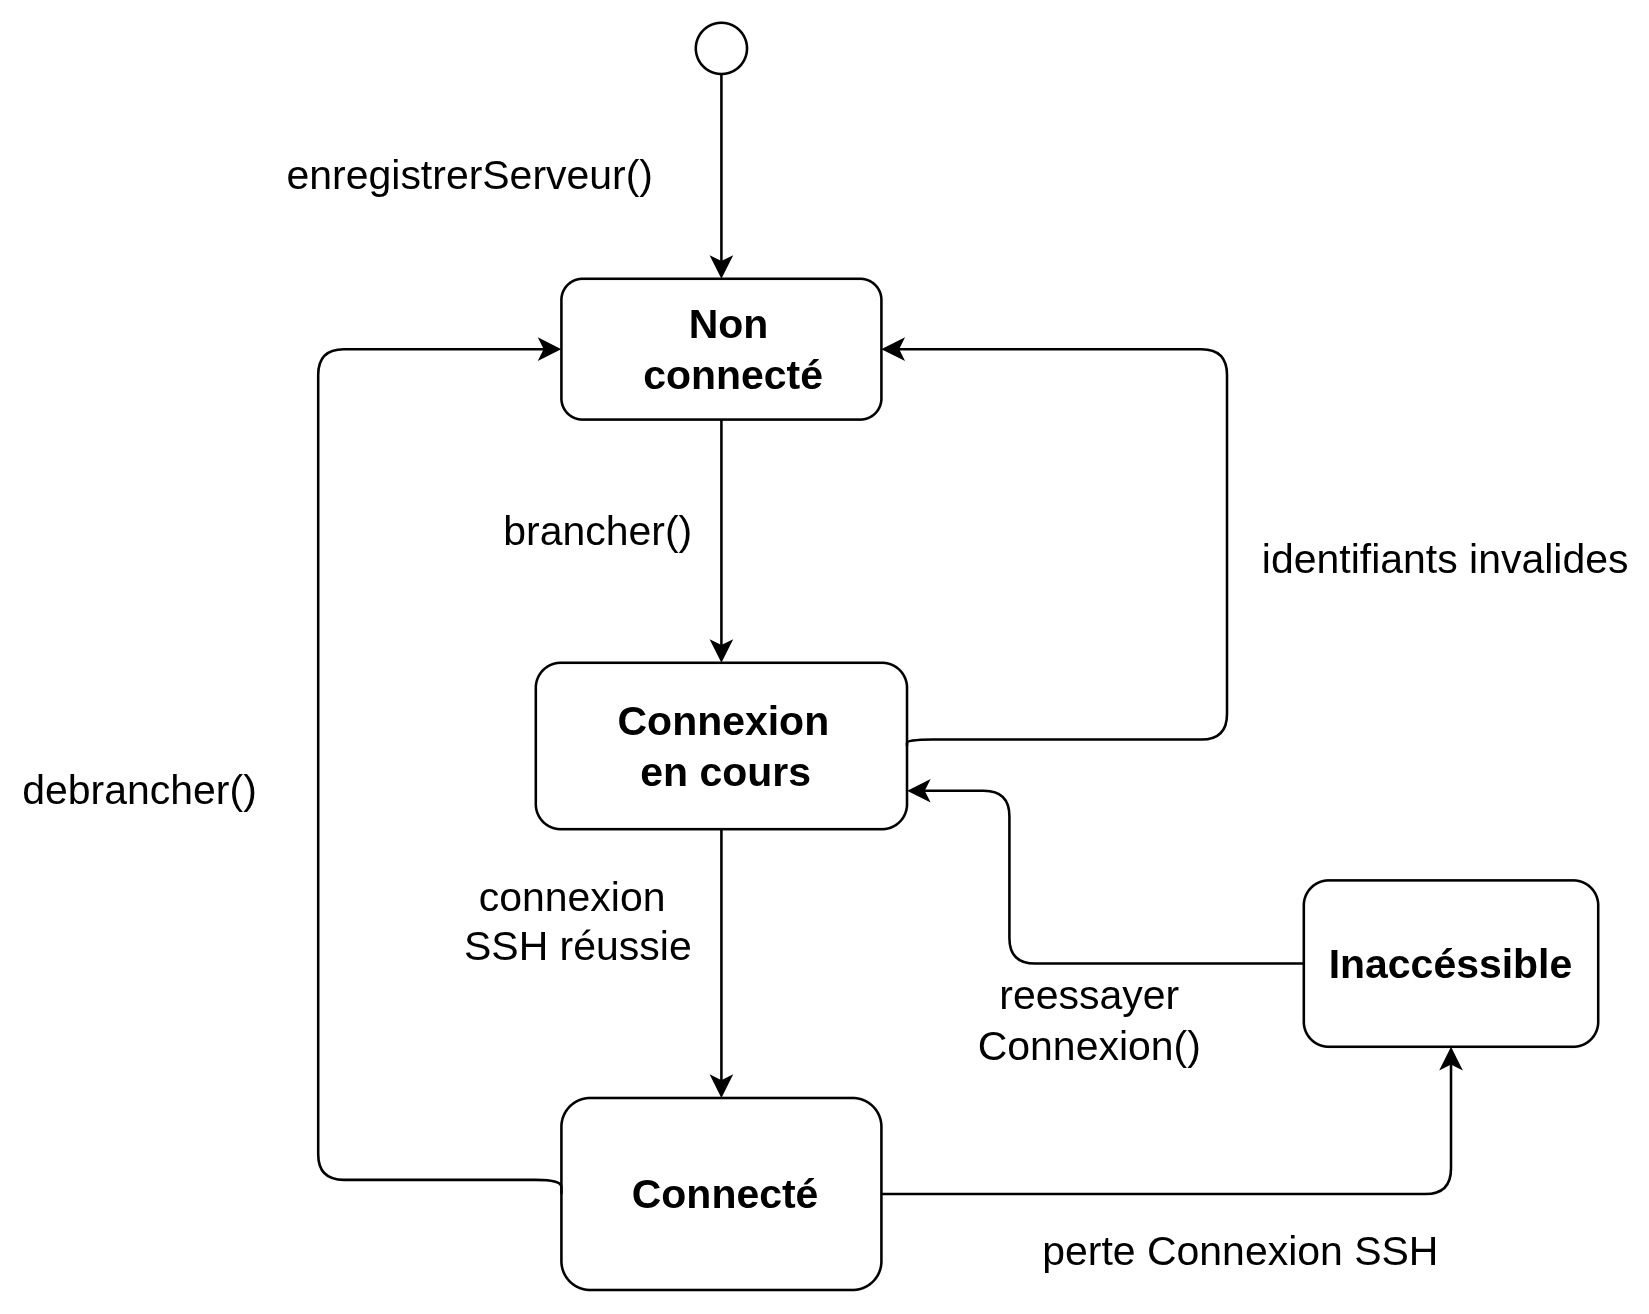
\includegraphics[width=\linewidth]{assets/diagrams/03-diagramme_ET_serveur.png}
  \caption{État-transition de la connectivité d'un serveur physique}
  \label{fig:etat-serveur}
\end{figure}

Ce second état-transition complète le précédent sur un point différent :
il ne modélise pas un flux métier, mais la disponibilité technique d'un
serveur. Trois états actifs se distinguent :

\begin{itemize}
  \item \texttt{Connecté} : état nominal, atteint après une connexion SSH
        réussie.
  \item \texttt{Inaccéssible} : atteint après une perte de connexion,
        avec une tentative de reconnexion possible sans repasser par un
        branchement complet.
  \item \texttt{Non\_connecté} : état initial, ou état de repli si les
        identifiants fournis sont invalides.
\end{itemize}

Un serveur inaccessible n'est donc pas retiré de l'inventaire : il reste
identifié comme tel, en attente d'une reconnexion, ce qui distingue une
panne réseau temporaire d'un débranchement volontaire.

\subsection{Résolution d'une permission}

\begin{figure}[H]
  \centering
  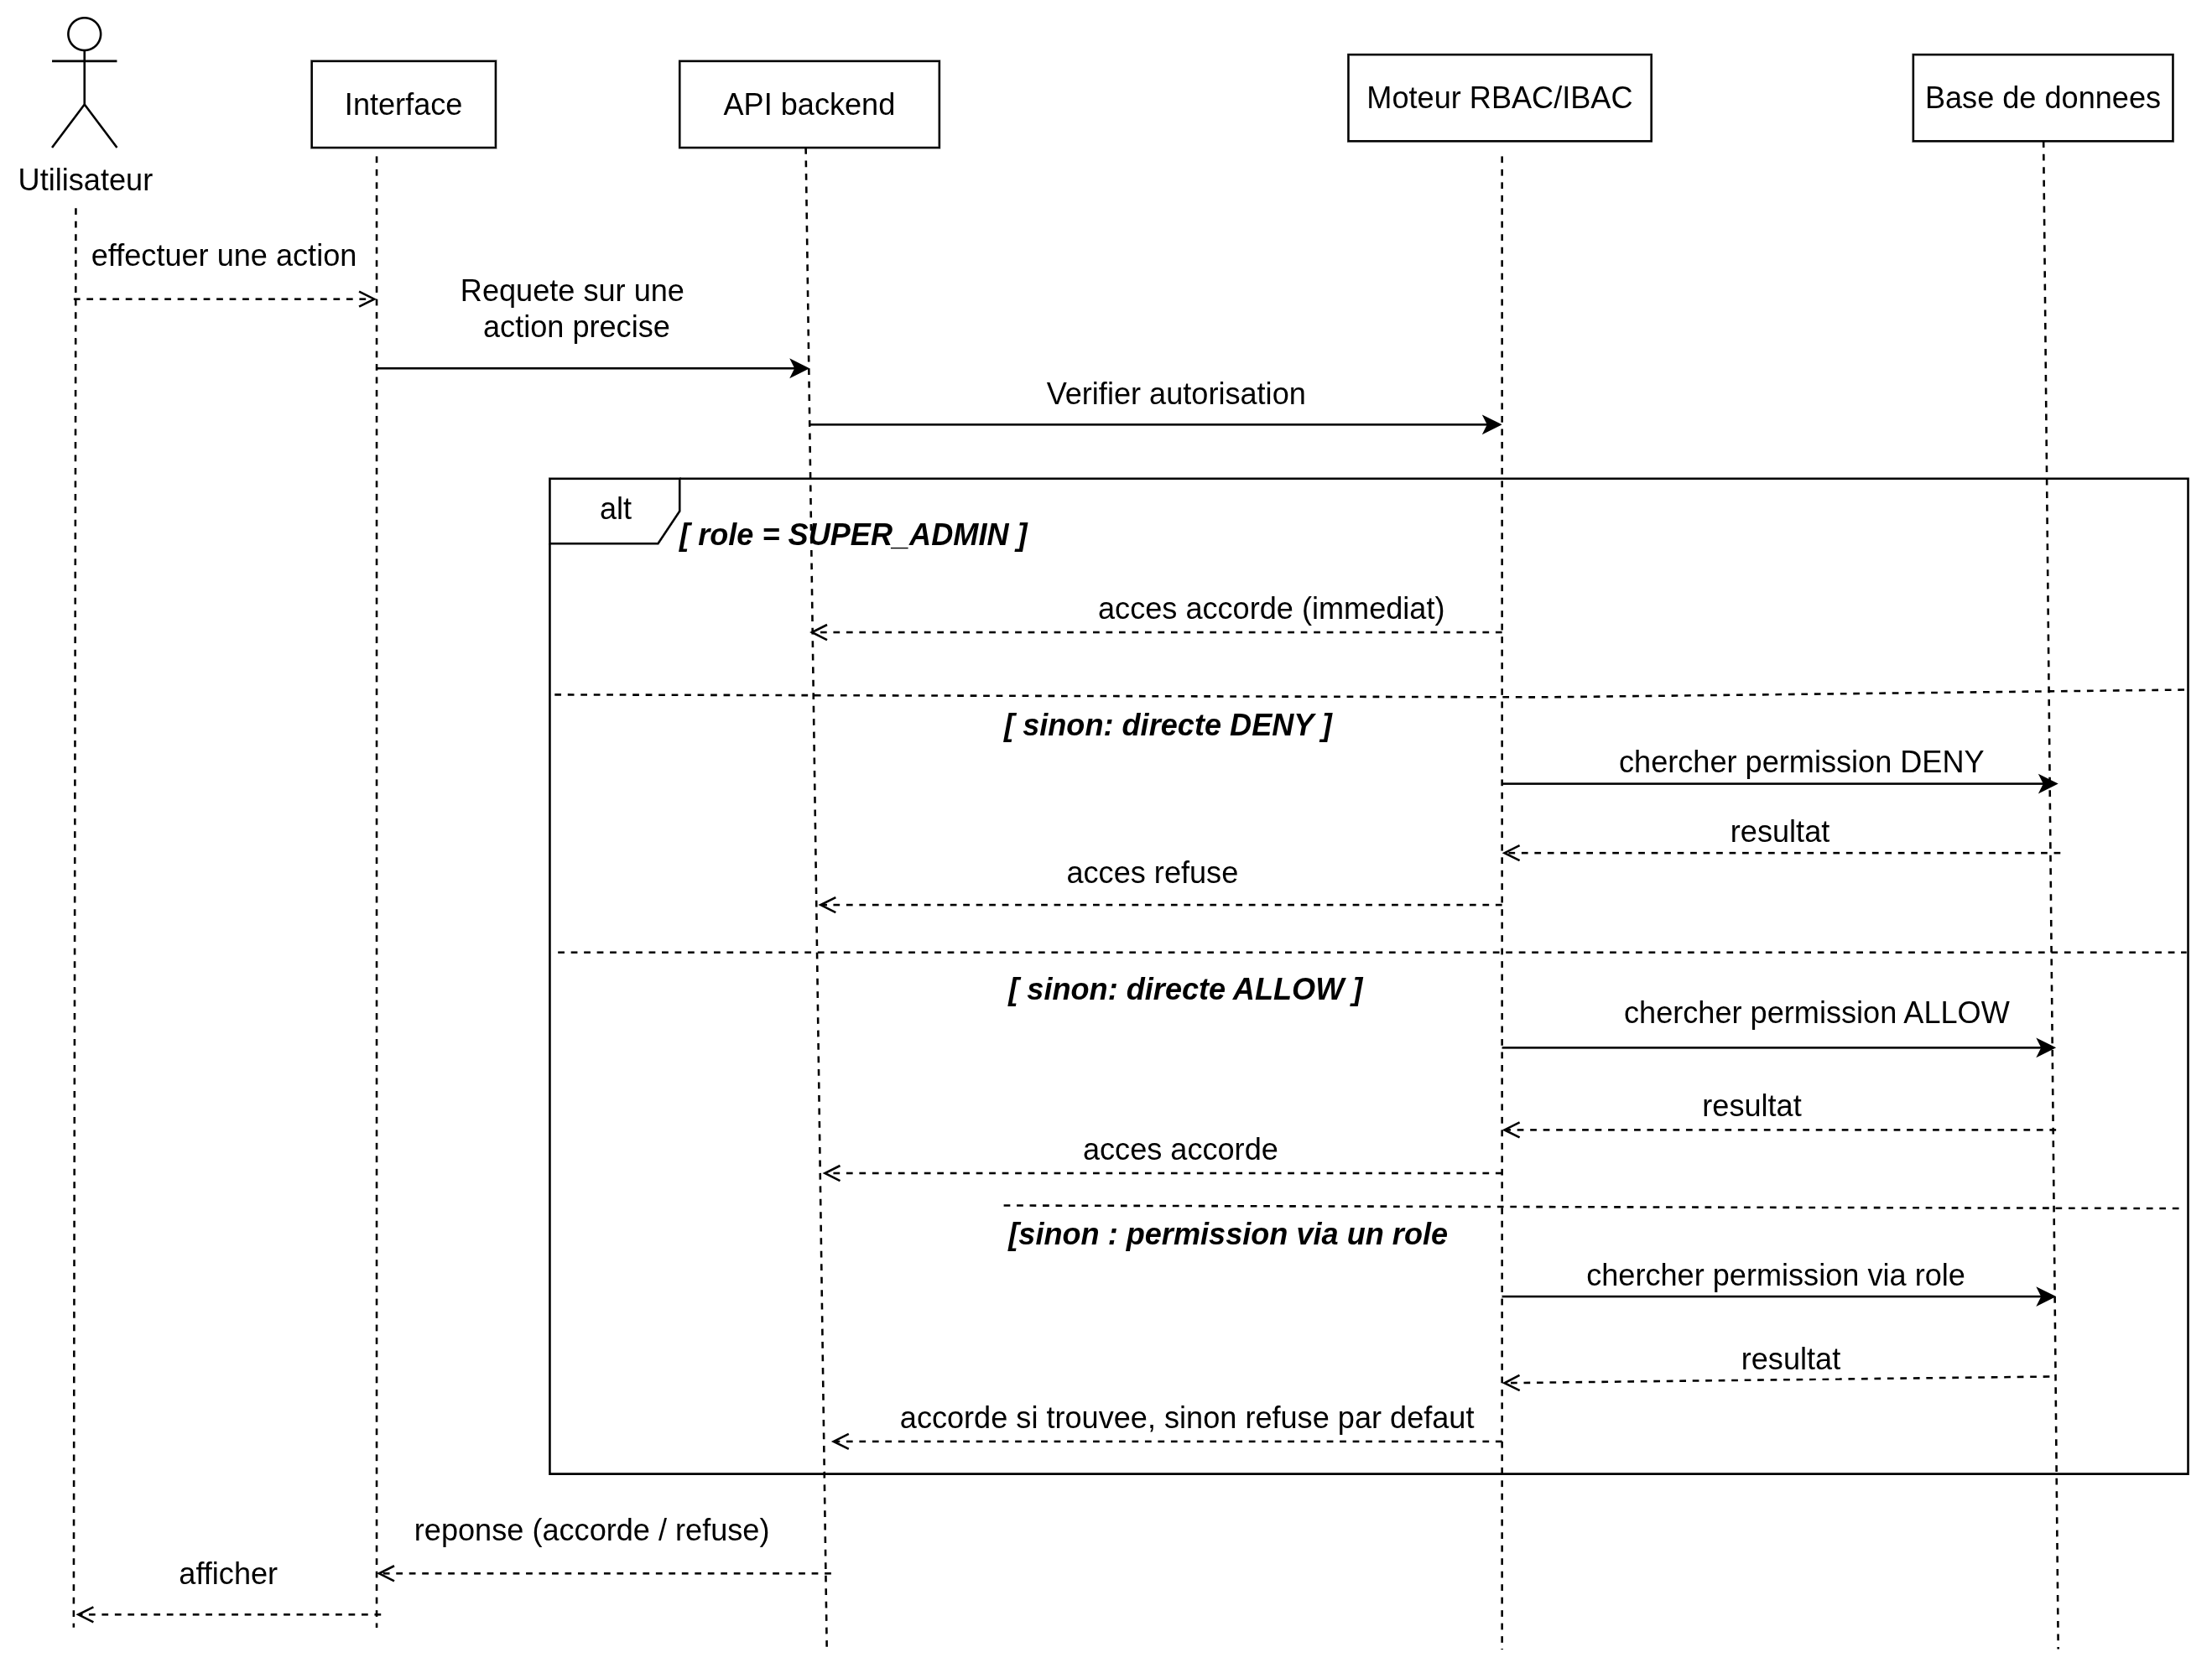
\includegraphics[width=\linewidth]{assets/diagrams/03-diagramme_seq_resolution_permission.png}
  \caption{Séquence de résolution d'une permission}
  \label{fig:sequence-permission}
\end{figure}

Cette séquence détaille, étape par étape, l'algorithme déjà décrit en
section~\ref{chap:etude-technique} de ce chapitre. Le point structurant
apparaît dans l'ordre des branches du fragment \textit{alt} : une
permission directe de refus est vérifiée avant toute permission
d'autorisation, qu'elle soit directe ou issue d'un rôle. Cet ordre
garantit qu'aucune combinaison de rôles, même la plus permissive, ne peut
contourner un refus explicite.

\subsection{Connexion d'un nouveau serveur}

\begin{figure}[H]
  \centering
  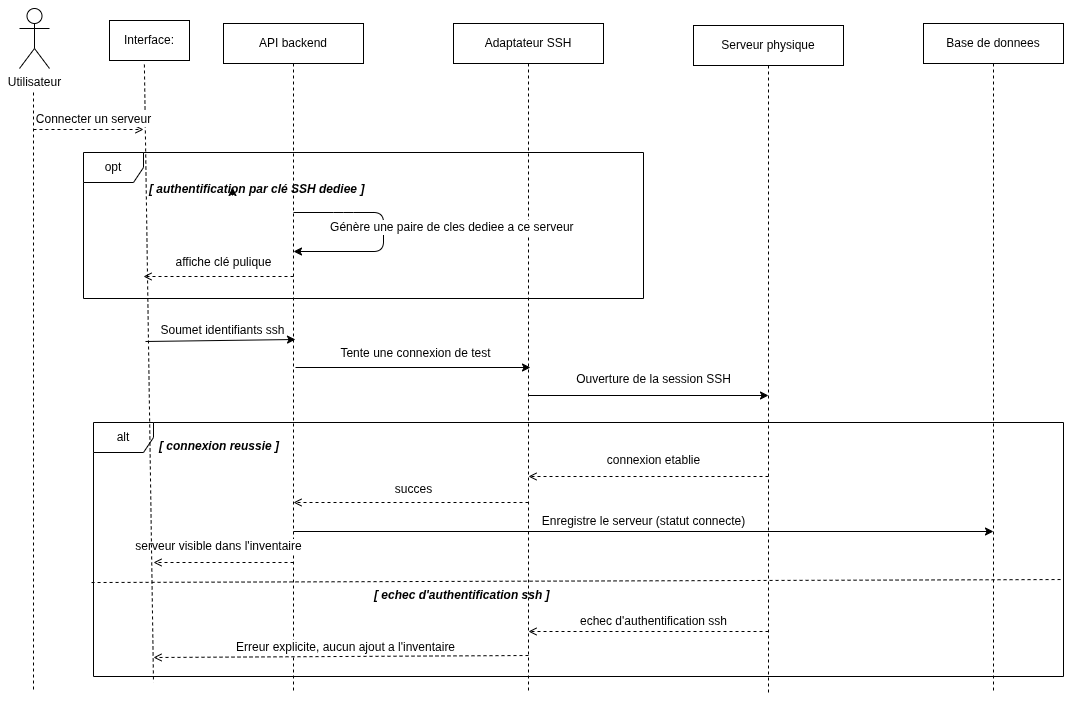
\includegraphics[width=\linewidth]{assets/diagrams/03-diagramme_seq_connexion_serveur.png}
  \caption{Séquence de connexion d'un nouveau serveur}
  \label{fig:sequence-connexion-serveur}
\end{figure}

Deux points de cette séquence méritent d'être soulignés :

\begin{itemize}
  \item La connexion est d'abord testée avant tout enregistrement en
        base : un serveur n'entre dans l'inventaire que si la connexion a
        réellement réussi.
  \item Le fragment optionnel de génération de clé dédiée montre une
        règle de sécurité déjà énoncée : une clé publique affichée sans
        installation dans le délai imparti est automatiquement invalidée
        et supprimée, sans intervention manuelle.
\end{itemize}

\subsection{Déploiement d'une application}

\begin{figure}[H]
  \centering
  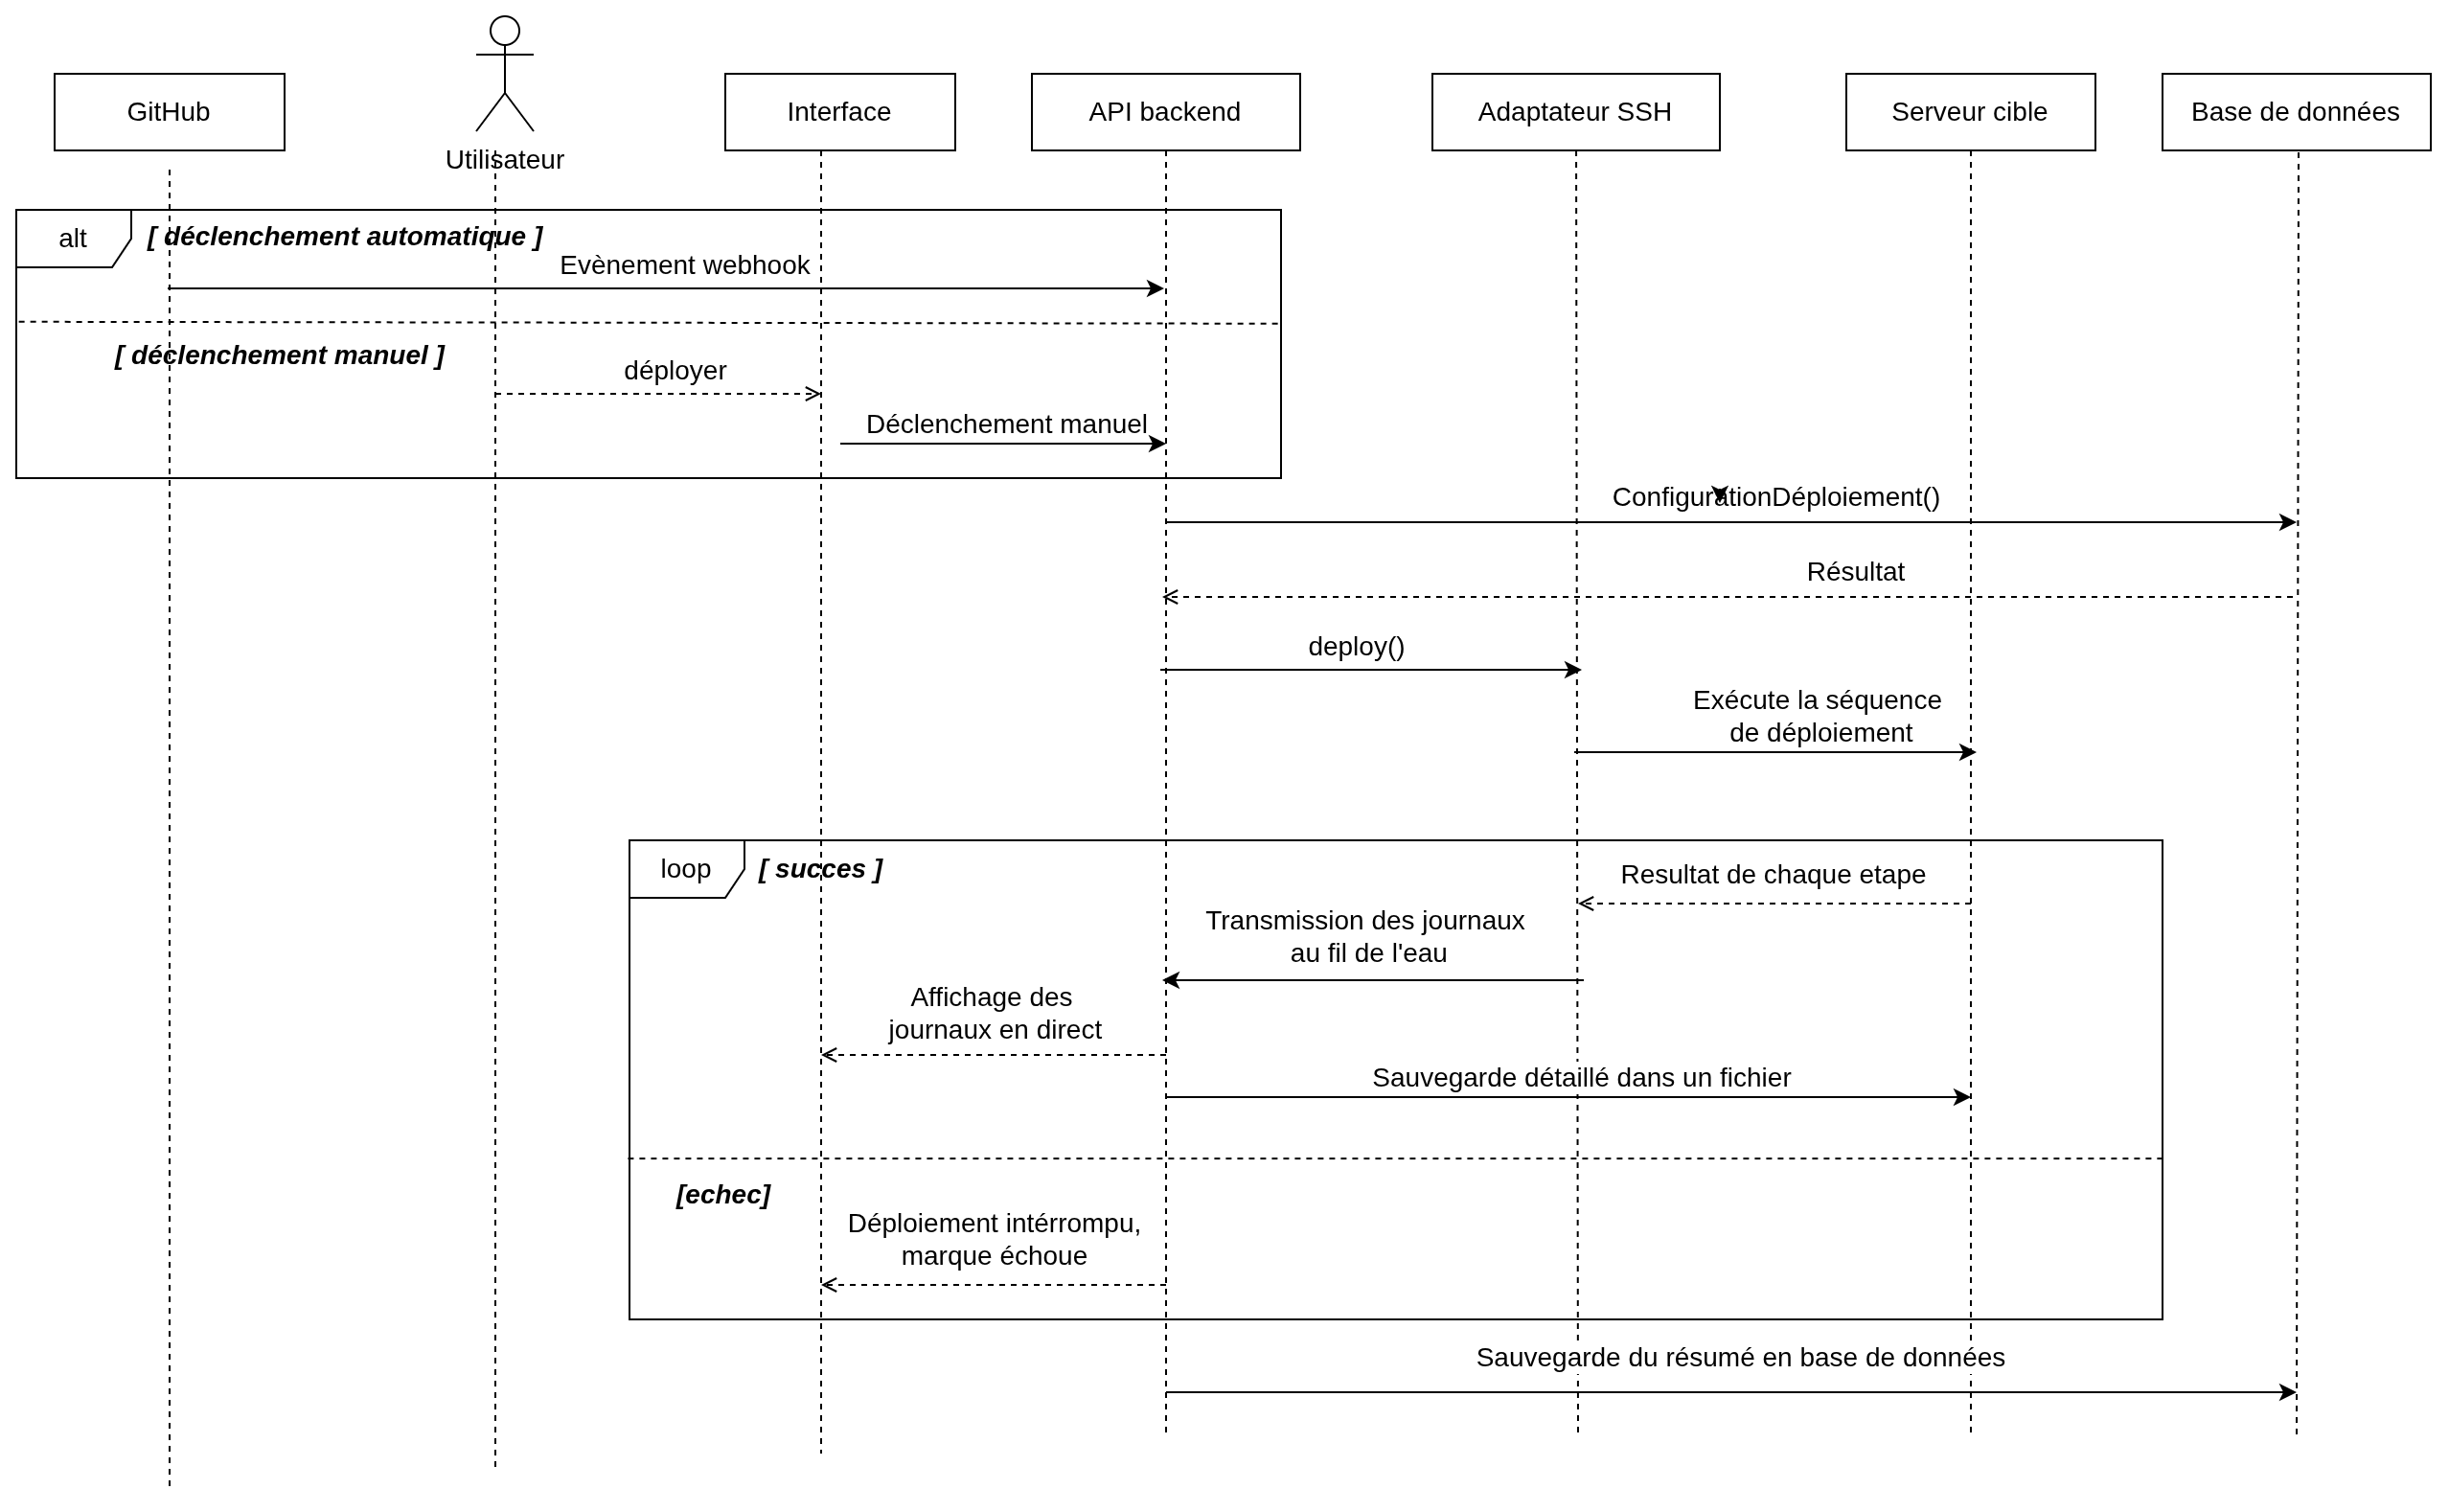
\includegraphics[width=\linewidth]{assets/diagrams/03-diagramme_seq_deploiement.png}
  \caption{Séquence de déploiement d'une application}
  \label{fig:sequence-deploiement}
\end{figure}

Cette séquence complète le cas d'utilisation détaillé en
section~\ref{chap:etude-technique} par l'ordre technique exact des
échanges. Trois points ressortent :

\begin{itemize}
  \item Le déclenchement automatique (webhook GitHub) et le déclenchement
        manuel convergent vers le même traitement dès que la
        configuration est validée : aucune différence de comportement
        n'existe entre les deux origines à partir de cette étape.
  \item Chaque étape de la séquence de déploiement transmet son résultat
        au fil de l'eau, diffusé en direct à l'utilisateur avant même la
        fin complète du déploiement.
  \item L'archivage suit une double écriture : le détail complet est
        sauvegardé dans un fichier, tandis qu'une synthèse est
        systématiquement écrite en base de données, y compris en cas
        d'échec.
\end{itemize}